%%%%%%%%%%%%%%%%%%%%%%%%%%%%%%%%%%%%%%%%%%%%%%%%%%%%%%%%%%%%%%%%%%%%%%%%
\section{A continuum model in which the KPZ formula is a theorem}\label{sec:continuum}
%%%%%%%%%%%%%%%%%%%%%%%%%%%%%%%%%%%%%%%%%%%%%%%%%%%%%%%%%%%%%%%%%%%%%%%%

The physical argument of Section~\ref{sec:surfaces} has two unproved steps for meanders: that
each curve acts like a spanning tree, and that the effects add up through the central charge.
This section describes a continuum model of random surfaces in which the second step is exact,
and explains the remaining ingredient, which Paper~D proves. In this section $N$ denotes a number
of squares, not the order of a meander.

\subsection{From counting to a continuum}\label{sec:dictionary}

The rest of the paper speaks the language of continuum random surfaces. This subsection explains
how that language translates the counting of Sections~\ref{sec:walks} and~\ref{sec:surfaces},
in three steps, and Table~\ref{tab:dictionary} collects the translation.

\emph{Step 1: describe a large surface by where its area sits.} Any sphere of squares can be
spread out over a round sphere in an essentially unique way that preserves angles (by the
uniformization theorem of complex analysis), much as a map of the Earth spreads the globe over a
flat page. After this, the surface is recorded by a single function on the round sphere: how
densely its squares are packed near each point. Write this density as $e^{\gamma h}$, where $h$
is a random function and $\gamma$ a number that sets how strongly $h$ is felt. For a uniformly
random sphere of squares, the logarithm of the density is predicted to be a \emph{Gaussian free
field}, the two-dimensional analog of Brownian motion described below. Intuitively, Brownian
motion records the ups and downs of a random walk, and the Gaussian free field records where a
random surface is crowded and where it is sparse.

\emph{Step 2: drawings change the law of the field.} Counting surfaces together with drawings
multiplies the weight of each surface by its number of drawings, which by~\eqref{eq:charge} is a
power of $\det\Delta_G$ up to a size factor. A classical formula of Polyakov says how this
determinant depends on the shape: its logarithm is a constant times the \emph{energy}
$\int|\nabla h|^2$ of the field, plus simpler terms that shift the field or depend only on the
size, without changing how much the field fluctuates. The weight of a Gaussian
field is itself of the form $e^{-\text{const}\cdot\int|\nabla h|^2}$. Multiplying one Gaussian
weight by another gives a Gaussian weight again, with a changed constant. So a drawing does not
change the kind of random surface; it only changes the parameter $\gamma$. Each spanning tree
changes it by the same amount, which is the additivity of $c$ in continuum form. Trees make the
field smoother, so $\gamma$ decreases: $\gamma^2=8/3$ for bare surfaces, $2$ with one tree, and
$(17-\sqrt{145})/3\approx1.653$ with two.

\emph{Step 3: read off the exponent from the size.} A counting law $\mu^n n^{-\alpha}$ becomes
a statement about the size of the surface: the total weight of surfaces of size at least $n$
decays like $n^{-(\alpha-1)}$ (Section~\ref{sec:surfaces}). In the continuum the size is a random
variable, and the question becomes how heavy its tail is. The growth rate $\mu$ has no continuum
counterpart: it counts local choices, and those are invisible after zooming out.

\begin{table}[ht]
\centering
\small
\renewcommand{\arraystretch}{1.15}
\begin{tabular}{p{0.47\textwidth}p{0.43\textwidth}}
\toprule
counting & continuum \\
\midrule
number of squares & area, or the number of squares of a random subdivision \\
uniformly random sphere of squares, $c=0$ & field with $\gamma^2=8/3$ (the Brownian map) \\
each sphere counted with its spanning trees, $c=-2$ & field with $\gamma^2=2$ \\
two tree-like drawings (a meander), $c=-4$ & field with $\gamma^2=(17-\sqrt{145})/3$ \\
a curve visiting every square once & a random curve through every point (SLE$_8$, Section~\ref{sec:limit}) \\
counting exponent $\alpha$ & one plus the tail exponent of the size, $1+4/\gamma^2$ \\
growth rate $\mu$ & no counterpart (a local quantity) \\
thin neck splitting a meander into halves & near-split of the two curves (Section~\ref{sec:limit}) \\
\bottomrule
\end{tabular}
\caption{A dictionary between counting and the continuum. Each entry on the right is a model or a
prediction, not a theorem about the entry on the left; the next subsections say which parts are
proved.}
\label{tab:dictionary}
\end{table}

The model below makes Steps~2 and~3 exact for a continuum surface built directly from a Gaussian
free field, with squares in place of area.

\subsection{Random surfaces from a random field}

The model is built from the \emph{Gaussian free field} $h$ on the sphere. It is a random
function whose values $h(z)$ and $h(w)$ at two points have covariance about $-\log|z-w|$, minus
the logarithm of their distance. It is too rough to have values at single points, since this
covariance is infinite at $z=w$, but its average $h_S$ over a square
$S$ is an ordinary normal random variable, with variance about $\log(1/|S|)$, where $|S|$ denotes
the side length of $S$. Intuitively, $h$ is the two-dimensional analog of Brownian motion. We use
it on a fixed unit square drawn on the sphere.

Fix a parameter $Q\ge2$ and a small number $\varepsilon>0$. Start from the unit square and repeat
the following rule: split a square $S$ into four equal squares if
\[ e^{h_S/Q}\,|S| \;>\; \varepsilon ,\]
and keep it otherwise. Let $N$ be the number of squares at the end. Intuitively,
$e^{h_S/Q}|S|$ is the size of $S$ as seen by the field. Where the field is high, squares count as
large and are split again and again, so high regions are covered by many small squares. Intuitively, the final squares play the role of the faces of a random planar map, and
$N$ is the size of the surface. The parameter $Q$ enters only through this rule; the field itself
does not depend on it. This construction is due to Ang, Park, Pfeffer and
Sheffield~\cite{APPS}, following earlier work on the same subdivisions~\cite{DS}.

The parameter $Q$ is tied to the central charge $c$ by $Q^2=(25-c)/6$, so $Q\ge2$ corresponds to
$c\le1$. This is how the physics literature matches $Q$ to $c$, and the next subsection shows why it
is natural: adding $k$ spanning trees raises $Q^2$ by $k/3$, which is exactly a drop of $2k$ in
$c$. The probability literature usually writes $Q$ through a second number $\gamma\in(0,2]$,
\begin{equation}\label{eq:Q}
Q^2 \;=\; \frac{25-c}{6}, \qquad Q \;=\; \frac{2}{\gamma}+\frac{\gamma}{2};
\end{equation}
of the two solutions $\gamma$ of the second equation we take the one in $(0,2]$. So $\gamma=2$ at
$Q=2$, and $\gamma\to0$ as $Q\to\infty$. A bare surface, $c=0$, has $Q^2=25/6$ and
$\gamma^2=8/3$; the meander value $c=-4$ has $Q^2=29/6$ and
$\gamma^2=(17-\sqrt{145})/3\approx1.653$. Squaring the second relation gives
$Q^2-2=4/\gamma^2+\gamma^2/4$, so with $x=4/\gamma^2$ it says exactly $x+1/x=(13-c)/6$. The KPZ
formula~\eqref{eq:kpz} is therefore the statement that the tail exponent $x$ equals $4/\gamma^2$.

\subsection{Drawings as an exact change of parameter}

For a planar map, the number of spanning trees equals a determinant built from the map's
Laplacian matrix, by Kirchhoff's theorem; equivalently, it is the product of the nonzero
eigenvalues of the Laplacian, divided by the number of vertices. The continuum model has an
analog. The Laplacian of a
continuum surface has infinitely many eigenvalues, so their product has to be renormalized; the
result is the \emph{regularized determinant}. Ang, Park, Pfeffer and Sheffield proved that
weighting the model by the $k$-th power of this determinant has exactly the same effect, for
surfaces with a given number of squares, as changing $Q^2$ to $Q^2+k/3$, that is, $c$ to
$c-2k$~\cite[Theorem~6.9]{APPS}. Intuitively, in this model drawing $k$ spanning trees is the
same as lowering the central charge by $2k$. The additivity of $c$, which is an assumption for
meanders, is here a theorem.

Write $Q_k$ for the parameter after the change, $Q_k^2=Q^2+k/3$. Their theorem compares
surfaces with the same number of squares. Comparing surfaces with different numbers of squares
needs two corrections, which Paper~D derives. The determinant contains a factor proportional to
$N^{1/3}$, which must be divided out. And the comparison of the two models is a Gaussian change of
variables, which contributes a factor $Q/Q_k$ for each square, so $(Q/Q_k)^N$ in all; one
multiplies by its inverse. This second factor is purely exponential in $N$: like $\mu^n$ for
meanders, it changes the growth rate but not the exponent.

\subsection{The tail law}

What was missing to read off an exponent is the distribution of the number of squares. It is
proved in Paper~D~\cite{PaperD}.

\begin{theorem}[Paper~D~\cite{PaperD}]\label{thm:tail}
For every $Q\ge2$ and every fixed $\varepsilon>0$,
\[ \lim_{n\to\infty}\frac{\log \Pr(N\ge n)}{\log n} \;=\; -\frac{4}{\gamma^2}, \]
with $\gamma$ given by~\eqref{eq:Q}.
\end{theorem}

Combined with the exact change of parameter, this gives the full KPZ curve.

\begin{theorem}[Paper~D~\cite{PaperD}]\label{thm:apps}
In the model above at $c=0$, with $Q_0^2=25/6$, weight each surface by the $k$-th power of the
regularized determinant, divided by $N^{k/3}$, and by the factor $(Q_k/Q_0)^N$ with
$Q_k^2=Q_0^2+k/3$. For every real $k\ge-1/2$, the total weight of surfaces with at least $n$
squares is $n^{-x_k+o(1)}$, where
\[ x_k+\frac1{x_k} \;=\; \frac{13+2k}{6},\qquad x_k\ge1 .\]
At $k=2$, the analog of two spanning trees, $x_2=(17+\sqrt{145})/12$, so
$1+x_2=\alpha_*$.
\end{theorem}

By the discussion after~\eqref{eq:kpz}, a tail exponent $x_2$ corresponds to the counting
exponent $1+x_2$. Two caveats keep this in proportion. The statement is about cumulative tails,
$\Pr(N\ge n)$, up to factors $n^{o(1)}$, not about the probability of each size. And it concerns
a continuum model in which the spanning trees are replaced by a determinant; it says nothing
directly about meanders, where the curves are actual curves on a discrete surface.

\subsection{Idea of the proof}\label{sec:tailidea}

We describe the upper bound for $Q>2$; the endpoint $Q=2$ needs a separate argument, given in
Paper~D. The number of squares is large only if the field is unusually high somewhere, since
high regions are where squares keep splitting. Count the squares of side $2^{-j}$ whose split
condition holds.
For a number $a>0$, the condition $e^{h_S/Q}2^{-j}>\varepsilon$ implies
$(e^{h_S/Q}2^{-j}/\varepsilon)^{aQ}>1$, and averaging over the $4^j$ squares at that depth shows
that their number is at most a constant times
\[ 2^{\,j\,(2-aQ+a^2/2)} \]
times a random factor whose $p$-th moment, the expected value of its $p$-th power, is finite for
every $p<4/a^2$. The exponent
$2-aQ+a^2/2$ is a quadratic in $a$ whose two roots are $\gamma$ and $4/\gamma$, as one checks from
$Q=2/\gamma+\gamma/2$. It is negative exactly between them. Choosing $a$ slightly above $\gamma$
makes the counts summable over $j$ and shows that the $p$-th moment of $N$ is finite for every
$p<4/\gamma^2$. By Markov's inequality, $\Pr(N\ge n)\le \mathbb E[N^p]\,n^{-p}$ for each such
order $p$, hence $\Pr(N\ge n)\le n^{-4/\gamma^2+o(1)}$. The matching lower bound comes from the
cheapest way to make $N$ large: raise the field over one small square, which happens with a
probability of the predicted size, and show that its descendants then produce enough squares.

The ratio of the two roots, $(4/\gamma)/\gamma=4/\gamma^2$, is exactly the KPZ number $x$. This
is where the quadratic of the physical prediction comes from in the proof.

\subsection{Area versus number of squares}\label{sec:area}

The surface also carries an area: the integral of $e^{\gamma h}$, suitably renormalized because
$h$ has no values at points. A square of side $|S|$ has area roughly $e^{\gamma h_S}|S|^{\gamma Q}$,
and the splitting rule $e^{h_S/Q}|S|>\varepsilon$ is the same as asking that this rough area
exceed $\varepsilon^{\gamma Q}$. So the rule splits squares until each has small area. A natural
first idea is that $N$ should be proportional to the area, whose tail is
known~\cite{RV,Wong}. For $Q>2$ this is false in a precise sense (Paper~D): given that the area is
very large, the probability that $N=1$ stays bounded away from zero. The field can be very high on
fine scales inside a square that the splitting rule never inspects, because the rule only looks
at averages over squares it has already created. The proof of Theorem~\ref{thm:tail} therefore
works with the squares directly.

\subsection{A branching random walk model}\label{sec:cascade}

A simpler model shows the mechanism in its purest form. Call
$H(S)=h_S+Q\log(|S|/\varepsilon)$ the \emph{height} of a square, so that $S$ is split exactly when
$H(S)>0$. Passing from a square to one of its four children lowers $Q\log|S|$ by $Q\log2$ and
changes $h_S$ by a random amount of variance about $\log2$. In the toy model these random amounts
are independent normal steps, independent for different children; in the model of
Section~\ref{sec:continuum} they are correlated. A square is split while its height is positive.
The squares then form a \emph{branching random walk killed at zero}: each square has four
children, each child's height is its parent's height plus a random step, and a square whose height
is not positive has no children. The number $N$ of final squares is determined by this family
tree, and for $Q>2$ its tail is known precisely~\cite{AHZ}:
\[ \Pr(N\ge n) \;\sim\; \mathrm{const}\cdot n^{-x}, \qquad x \;=\; \frac{\lambda_+}{\lambda_-},
\qquad \lambda_\pm \;=\; Q\pm\sqrt{Q^2-4}. \]
The two rates are the roots of Section~\ref{sec:tailidea}: $\lambda_-=\gamma$ and
$\lambda_+=4/\gamma$. Since $\lambda_+\lambda_-=4$ and $\lambda_++\lambda_-=2Q$,
\[ x+\frac1x \;=\; \frac{\lambda_+^2+\lambda_-^2}{\lambda_+\lambda_-} \;=\; Q^2-2 \;=\; \frac{13-c}{6} .\]
So the KPZ quadratic is the relation between the two exponential rates of a killed branching
random walk. In this toy model Paper~D also proves the local version: for $Q>2$, every
starting height and every $n$ that is one more than a multiple of $3$ (the only possible values,
since each split adds three squares), $\Pr(N=n)$ lies between two constant multiples of
$n^{-1-x}$. At $Q^2=29/6$ the
exponent $1+x$ is again $\alpha_*$.

%%%%%%%%%%%%%%%%%%%%%%%%%%%%%%%%%%%%%%%%%%%%%%%%%%%%%%%%%%%%%%%%%%%%%%%%
\section{The conjectured limit of large meanders}\label{sec:limit}
%%%%%%%%%%%%%%%%%%%%%%%%%%%%%%%%%%%%%%%%%%%%%%%%%%%%%%%%%%%%%%%%%%%%%%%%

\subsection{The conjecture}

Borga, Gwynne and Sun proposed a precise description of what a large uniformly random meander
looks like when zoomed out~\cite{BGS}. It has four ingredients.

\begin{itemize}
\item \emph{The surface} is a \emph{Liouville quantum gravity sphere} (the name comes from
physics): a continuum random surface of total area one, built from the Gaussian free field as in
Section~\ref{sec:continuum}, with the size of a region measured by the area $\int e^{\gamma h}$ of
Section~\ref{sec:area} instead of by counting squares. Its parameter is
$\gamma^2=(17-\sqrt{145})/3$, the value that~\eqref{eq:Q} assigns to $c=-4$.
\item \emph{The river and the road} become two random curves. Recall that each of them visits
every square of the sphere exactly once. When the squares become infinitely small, such a curve
becomes a continuous curve that passes through every point of the surface, like the
space-filling curves of Peano and Hilbert, but random. Which random curve it is, is known for
spanning trees (Figure~\ref{fig:peano}). Walk around a spanning tree of a fine grid, keeping the
tree on your left. This path visits the neighborhood of every vertex and returns to its start,
and as the grid gets finer it converges to a particular random space-filling curve, called
SLE$_8$~\cite{LSWust}. (SLE, for Schramm--Loewner evolution, is a family of random curves indexed
by a number; the value $8$ gives the curve that fills space.) Since the river and the road are
expected to behave like spanning trees (Section~\ref{sec:charge}), both become SLE$_8$ curves.
\item \emph{The two curves are independent} of each other and of the surface. Intuitively,
zoomed out, knowing the river tells nothing about the road. This is the continuum form of the
assumption that the two central charges add.
\item \emph{Time along each curve is measured by area}: by time $t$ the curve has covered area $t$,
and it covers the whole surface by time one. This is the continuum version of numbering the
crossings: the $i$-th crossing along the river corresponds to time about $i/(2n)$ along the
river curve, and similarly for the road.
\end{itemize}

\begin{figure}[ht]
\centering
% Path around a random spanning tree (Wilsons algorithm); generated by a script.
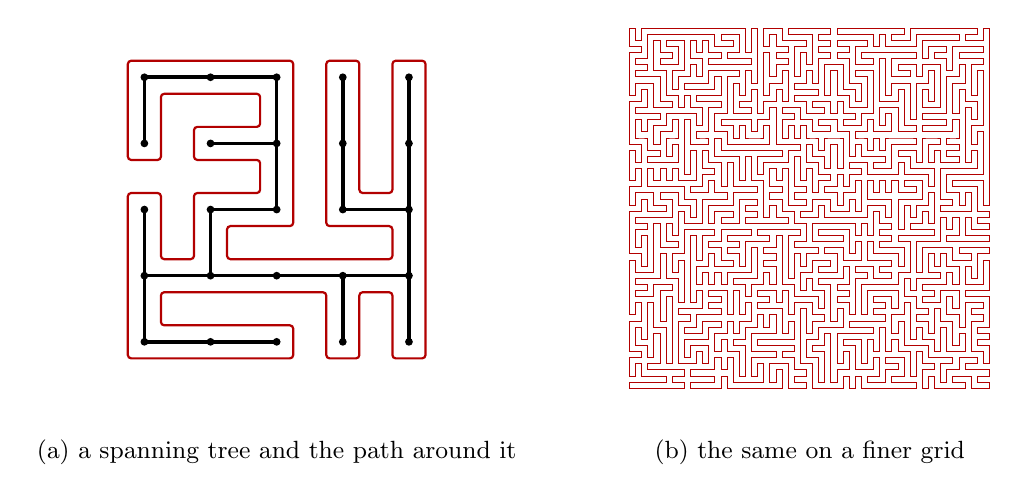
\begin{tikzpicture}
\begin{scope}[x=0.420cm,y=0.420cm,yshift=0.55cm]
  \draw[red!70!black,line width=0.8pt,rounded corners=1.2pt] (3.5,-0.5) -- (4.5,-0.5) -- (4.5,0.5) -- (3.5,0.5) -- (2.5,0.5) -- (1.5,0.5) -- (0.5,0.5) -- (0.5,1.5) -- (1.5,1.5) -- (2.5,1.5) -- (3.5,1.5) -- (4.5,1.5) -- (5.5,1.5) -- (5.5,0.5) -- (5.5,-0.5) -- (6.5,-0.5) -- (6.5,0.5) -- (6.5,1.5) -- (7.5,1.5) -- (7.5,0.5) -- (7.5,-0.5) -- (8.5,-0.5) -- (8.5,0.5) -- (8.5,1.5) -- (8.5,2.5) -- (8.5,3.5) -- (8.5,4.5) -- (8.5,5.5) -- (8.5,6.5) -- (8.5,7.5) -- (8.5,8.5) -- (7.5,8.5) -- (7.5,7.5) -- (7.5,6.5) -- (7.5,5.5) -- (7.5,4.5) -- (6.5,4.5) -- (6.5,5.5) -- (6.5,6.5) -- (6.5,7.5) -- (6.5,8.5) -- (5.5,8.5) -- (5.5,7.5) -- (5.5,6.5) -- (5.5,5.5) -- (5.5,4.5) -- (5.5,3.5) -- (6.5,3.5) -- (7.5,3.5) -- (7.5,2.5) -- (6.5,2.5) -- (5.5,2.5) -- (4.5,2.5) -- (3.5,2.5) -- (2.5,2.5) -- (2.5,3.5) -- (3.5,3.5) -- (4.5,3.5) -- (4.5,4.5) -- (4.5,5.5) -- (4.5,6.5) -- (4.5,7.5) -- (4.5,8.5) -- (3.5,8.5) -- (2.5,8.5) -- (1.5,8.5) -- (0.5,8.5) -- (-0.5,8.5) -- (-0.5,7.5) -- (-0.5,6.5) -- (-0.5,5.5) -- (0.5,5.5) -- (0.5,6.5) -- (0.5,7.5) -- (1.5,7.5) -- (2.5,7.5) -- (3.5,7.5) -- (3.5,6.5) -- (2.5,6.5) -- (1.5,6.5) -- (1.5,5.5) -- (2.5,5.5) -- (3.5,5.5) -- (3.5,4.5) -- (2.5,4.5) -- (1.5,4.5) -- (1.5,3.5) -- (1.5,2.5) -- (0.5,2.5) -- (0.5,3.5) -- (0.5,4.5) -- (-0.5,4.5) -- (-0.5,3.5) -- (-0.5,2.5) -- (-0.5,1.5) -- (-0.5,0.5) -- (-0.5,-0.5) -- (0.5,-0.5) -- (1.5,-0.5) -- (2.5,-0.5) -- cycle;
  \draw[line width=1.3pt] (0,2)--(0,0);
  \draw[line width=1.3pt] (0,4)--(0,2);
  \draw[line width=1.3pt] (0,6)--(0,8);
  \draw[line width=1.3pt] (0,8)--(2,8);
  \draw[line width=1.3pt] (2,8)--(4,8);
  \draw[line width=1.3pt] (4,8)--(4,6);
  \draw[line width=1.3pt] (4,6)--(4,4);
  \draw[line width=1.3pt] (4,4)--(2,4);
  \draw[line width=1.3pt] (2,4)--(2,2);
  \draw[line width=1.3pt] (2,2)--(0,2);
  \draw[line width=1.3pt] (2,0)--(0,0);
  \draw[line width=1.3pt] (2,6)--(4,6);
  \draw[line width=1.3pt] (4,0)--(2,0);
  \draw[line width=1.3pt] (4,2)--(2,2);
  \draw[line width=1.3pt] (6,0)--(6,2);
  \draw[line width=1.3pt] (6,2)--(4,2);
  \draw[line width=1.3pt] (6,4)--(8,4);
  \draw[line width=1.3pt] (8,4)--(8,2);
  \draw[line width=1.3pt] (8,2)--(6,2);
  \draw[line width=1.3pt] (6,6)--(6,4);
  \draw[line width=1.3pt] (6,8)--(6,6);
  \draw[line width=1.3pt] (8,0)--(8,2);
  \draw[line width=1.3pt] (8,6)--(8,4);
  \draw[line width=1.3pt] (8,8)--(8,6);
  \foreach \i in {0,...,4} \foreach \j in {0,...,4} \fill (2*\i,2*\j) circle[radius=1.4pt];
\end{scope}
\begin{scope}[xshift=6.2cm]
\begin{scope}[x=0.0775cm,y=0.0775cm]
  \draw[red!70!black,line width=0.35pt] (26.5,20.5) -- (26.5,21.5) -- (27.5,21.5) -- (27.5,20.5) -- (27.5,19.5) -- (28.5,19.5) -- (28.5,20.5) -- (28.5,21.5) -- (29.5,21.5) -- (30.5,21.5) -- (30.5,22.5) -- (29.5,22.5) -- (28.5,22.5) -- (27.5,22.5) -- (26.5,22.5) -- (26.5,23.5) -- (27.5,23.5) -- (28.5,23.5) -- (28.5,24.5) -- (28.5,25.5) -- (28.5,26.5) -- (27.5,26.5) -- (26.5,26.5) -- (26.5,27.5) -- (26.5,28.5) -- (25.5,28.5) -- (24.5,28.5) -- (24.5,29.5) -- (24.5,30.5) -- (23.5,30.5) -- (22.5,30.5) -- (22.5,31.5) -- (23.5,31.5) -- (24.5,31.5) -- (24.5,32.5) -- (23.5,32.5) -- (22.5,32.5) -- (22.5,33.5) -- (22.5,34.5) -- (22.5,35.5) -- (23.5,35.5) -- (23.5,34.5) -- (23.5,33.5) -- (24.5,33.5) -- (24.5,34.5) -- (24.5,35.5) -- (25.5,35.5) -- (25.5,34.5) -- (25.5,33.5) -- (25.5,32.5) -- (25.5,31.5) -- (25.5,30.5) -- (25.5,29.5) -- (26.5,29.5) -- (27.5,29.5) -- (28.5,29.5) -- (28.5,30.5) -- (27.5,30.5) -- (26.5,30.5) -- (26.5,31.5) -- (27.5,31.5) -- (28.5,31.5) -- (28.5,32.5) -- (27.5,32.5) -- (26.5,32.5) -- (26.5,33.5) -- (26.5,34.5) -- (26.5,35.5) -- (26.5,36.5) -- (26.5,37.5) -- (27.5,37.5) -- (27.5,36.5) -- (27.5,35.5) -- (27.5,34.5) -- (27.5,33.5) -- (28.5,33.5) -- (28.5,34.5) -- (28.5,35.5) -- (29.5,35.5) -- (29.5,34.5) -- (29.5,33.5) -- (29.5,32.5) -- (29.5,31.5) -- (30.5,31.5) -- (30.5,32.5) -- (30.5,33.5) -- (31.5,33.5) -- (32.5,33.5) -- (32.5,34.5) -- (31.5,34.5) -- (30.5,34.5) -- (30.5,35.5) -- (30.5,36.5) -- (29.5,36.5) -- (28.5,36.5) -- (28.5,37.5) -- (28.5,38.5) -- (28.5,39.5) -- (29.5,39.5) -- (29.5,38.5) -- (29.5,37.5) -- (30.5,37.5) -- (31.5,37.5) -- (31.5,36.5) -- (31.5,35.5) -- (32.5,35.5) -- (32.5,36.5) -- (32.5,37.5) -- (32.5,38.5) -- (32.5,39.5) -- (33.5,39.5) -- (33.5,38.5) -- (33.5,37.5) -- (33.5,36.5) -- (33.5,35.5) -- (34.5,35.5) -- (34.5,36.5) -- (34.5,37.5) -- (34.5,38.5) -- (34.5,39.5) -- (34.5,40.5) -- (33.5,40.5) -- (32.5,40.5) -- (31.5,40.5) -- (31.5,39.5) -- (31.5,38.5) -- (30.5,38.5) -- (30.5,39.5) -- (30.5,40.5) -- (29.5,40.5) -- (28.5,40.5) -- (28.5,41.5) -- (28.5,42.5) -- (27.5,42.5) -- (27.5,41.5) -- (27.5,40.5) -- (26.5,40.5) -- (26.5,41.5) -- (26.5,42.5) -- (25.5,42.5) -- (25.5,41.5) -- (25.5,40.5) -- (24.5,40.5) -- (24.5,41.5) -- (24.5,42.5) -- (24.5,43.5) -- (25.5,43.5) -- (26.5,43.5) -- (26.5,44.5) -- (25.5,44.5) -- (24.5,44.5) -- (24.5,45.5) -- (25.5,45.5) -- (26.5,45.5) -- (27.5,45.5) -- (27.5,44.5) -- (27.5,43.5) -- (28.5,43.5) -- (29.5,43.5) -- (29.5,42.5) -- (29.5,41.5) -- (30.5,41.5) -- (31.5,41.5) -- (32.5,41.5) -- (32.5,42.5) -- (31.5,42.5) -- (30.5,42.5) -- (30.5,43.5) -- (31.5,43.5) -- (32.5,43.5) -- (33.5,43.5) -- (33.5,42.5) -- (33.5,41.5) -- (34.5,41.5) -- (35.5,41.5) -- (35.5,40.5) -- (35.5,39.5) -- (35.5,38.5) -- (35.5,37.5) -- (36.5,37.5) -- (36.5,38.5) -- (36.5,39.5) -- (37.5,39.5) -- (37.5,38.5) -- (37.5,37.5) -- (38.5,37.5) -- (39.5,37.5) -- (40.5,37.5) -- (41.5,37.5) -- (41.5,36.5) -- (40.5,36.5) -- (39.5,36.5) -- (39.5,35.5) -- (40.5,35.5) -- (41.5,35.5) -- (42.5,35.5) -- (42.5,36.5) -- (42.5,37.5) -- (42.5,38.5) -- (42.5,39.5) -- (43.5,39.5) -- (44.5,39.5) -- (45.5,39.5) -- (46.5,39.5) -- (46.5,40.5) -- (45.5,40.5) -- (44.5,40.5) -- (43.5,40.5) -- (42.5,40.5) -- (41.5,40.5) -- (41.5,39.5) -- (41.5,38.5) -- (40.5,38.5) -- (40.5,39.5) -- (40.5,40.5) -- (39.5,40.5) -- (39.5,39.5) -- (39.5,38.5) -- (38.5,38.5) -- (38.5,39.5) -- (38.5,40.5) -- (37.5,40.5) -- (36.5,40.5) -- (36.5,41.5) -- (37.5,41.5) -- (38.5,41.5) -- (38.5,42.5) -- (38.5,43.5) -- (39.5,43.5) -- (39.5,42.5) -- (39.5,41.5) -- (40.5,41.5) -- (41.5,41.5) -- (42.5,41.5) -- (42.5,42.5) -- (42.5,43.5) -- (42.5,44.5) -- (41.5,44.5) -- (41.5,43.5) -- (41.5,42.5) -- (40.5,42.5) -- (40.5,43.5) -- (40.5,44.5) -- (40.5,45.5) -- (41.5,45.5) -- (42.5,45.5) -- (43.5,45.5) -- (43.5,44.5) -- (43.5,43.5) -- (43.5,42.5) -- (43.5,41.5) -- (44.5,41.5) -- (45.5,41.5) -- (46.5,41.5) -- (46.5,42.5) -- (45.5,42.5) -- (44.5,42.5) -- (44.5,43.5) -- (44.5,44.5) -- (44.5,45.5) -- (44.5,46.5) -- (44.5,47.5) -- (44.5,48.5) -- (43.5,48.5) -- (43.5,47.5) -- (43.5,46.5) -- (42.5,46.5) -- (41.5,46.5) -- (40.5,46.5) -- (40.5,47.5) -- (40.5,48.5) -- (40.5,49.5) -- (40.5,50.5) -- (40.5,51.5) -- (40.5,52.5) -- (40.5,53.5) -- (41.5,53.5) -- (41.5,52.5) -- (41.5,51.5) -- (41.5,50.5) -- (41.5,49.5) -- (41.5,48.5) -- (41.5,47.5) -- (42.5,47.5) -- (42.5,48.5) -- (42.5,49.5) -- (43.5,49.5) -- (44.5,49.5) -- (45.5,49.5) -- (45.5,48.5) -- (45.5,47.5) -- (45.5,46.5) -- (45.5,45.5) -- (45.5,44.5) -- (45.5,43.5) -- (46.5,43.5) -- (46.5,44.5) -- (46.5,45.5) -- (46.5,46.5) -- (46.5,47.5) -- (46.5,48.5) -- (46.5,49.5) -- (47.5,49.5) -- (48.5,49.5) -- (48.5,50.5) -- (48.5,51.5) -- (49.5,51.5) -- (49.5,50.5) -- (49.5,49.5) -- (49.5,48.5) -- (49.5,47.5) -- (49.5,46.5) -- (48.5,46.5) -- (48.5,47.5) -- (48.5,48.5) -- (47.5,48.5) -- (47.5,47.5) -- (47.5,46.5) -- (47.5,45.5) -- (48.5,45.5) -- (49.5,45.5) -- (50.5,45.5) -- (50.5,46.5) -- (50.5,47.5) -- (50.5,48.5) -- (50.5,49.5) -- (50.5,50.5) -- (50.5,51.5) -- (50.5,52.5) -- (49.5,52.5) -- (48.5,52.5) -- (47.5,52.5) -- (47.5,51.5) -- (47.5,50.5) -- (46.5,50.5) -- (46.5,51.5) -- (46.5,52.5) -- (45.5,52.5) -- (44.5,52.5) -- (43.5,52.5) -- (43.5,51.5) -- (44.5,51.5) -- (45.5,51.5) -- (45.5,50.5) -- (44.5,50.5) -- (43.5,50.5) -- (42.5,50.5) -- (42.5,51.5) -- (42.5,52.5) -- (42.5,53.5) -- (43.5,53.5) -- (44.5,53.5) -- (45.5,53.5) -- (46.5,53.5) -- (46.5,54.5) -- (45.5,54.5) -- (44.5,54.5) -- (43.5,54.5) -- (42.5,54.5) -- (41.5,54.5) -- (40.5,54.5) -- (39.5,54.5) -- (38.5,54.5) -- (37.5,54.5) -- (37.5,53.5) -- (38.5,53.5) -- (39.5,53.5) -- (39.5,52.5) -- (38.5,52.5) -- (37.5,52.5) -- (36.5,52.5) -- (36.5,53.5) -- (36.5,54.5) -- (36.5,55.5) -- (37.5,55.5) -- (38.5,55.5) -- (38.5,56.5) -- (37.5,56.5) -- (36.5,56.5) -- (35.5,56.5) -- (34.5,56.5) -- (33.5,56.5) -- (33.5,55.5) -- (34.5,55.5) -- (35.5,55.5) -- (35.5,54.5) -- (34.5,54.5) -- (33.5,54.5) -- (33.5,53.5) -- (34.5,53.5) -- (35.5,53.5) -- (35.5,52.5) -- (35.5,51.5) -- (35.5,50.5) -- (35.5,49.5) -- (36.5,49.5) -- (37.5,49.5) -- (37.5,48.5) -- (37.5,47.5) -- (37.5,46.5) -- (36.5,46.5) -- (36.5,47.5) -- (36.5,48.5) -- (35.5,48.5) -- (34.5,48.5) -- (34.5,49.5) -- (34.5,50.5) -- (34.5,51.5) -- (34.5,52.5) -- (33.5,52.5) -- (32.5,52.5) -- (31.5,52.5) -- (31.5,51.5) -- (31.5,50.5) -- (31.5,49.5) -- (31.5,48.5) -- (31.5,47.5) -- (32.5,47.5) -- (32.5,48.5) -- (32.5,49.5) -- (32.5,50.5) -- (32.5,51.5) -- (33.5,51.5) -- (33.5,50.5) -- (33.5,49.5) -- (33.5,48.5) -- (33.5,47.5) -- (34.5,47.5) -- (35.5,47.5) -- (35.5,46.5) -- (35.5,45.5) -- (36.5,45.5) -- (37.5,45.5) -- (38.5,45.5) -- (38.5,46.5) -- (38.5,47.5) -- (38.5,48.5) -- (38.5,49.5) -- (38.5,50.5) -- (37.5,50.5) -- (36.5,50.5) -- (36.5,51.5) -- (37.5,51.5) -- (38.5,51.5) -- (39.5,51.5) -- (39.5,50.5) -- (39.5,49.5) -- (39.5,48.5) -- (39.5,47.5) -- (39.5,46.5) -- (39.5,45.5) -- (39.5,44.5) -- (38.5,44.5) -- (37.5,44.5) -- (37.5,43.5) -- (37.5,42.5) -- (36.5,42.5) -- (35.5,42.5) -- (34.5,42.5) -- (34.5,43.5) -- (35.5,43.5) -- (36.5,43.5) -- (36.5,44.5) -- (35.5,44.5) -- (34.5,44.5) -- (34.5,45.5) -- (34.5,46.5) -- (33.5,46.5) -- (33.5,45.5) -- (33.5,44.5) -- (32.5,44.5) -- (32.5,45.5) -- (32.5,46.5) -- (31.5,46.5) -- (30.5,46.5) -- (29.5,46.5) -- (29.5,45.5) -- (30.5,45.5) -- (31.5,45.5) -- (31.5,44.5) -- (30.5,44.5) -- (29.5,44.5) -- (28.5,44.5) -- (28.5,45.5) -- (28.5,46.5) -- (27.5,46.5) -- (26.5,46.5) -- (26.5,47.5) -- (27.5,47.5) -- (28.5,47.5) -- (29.5,47.5) -- (30.5,47.5) -- (30.5,48.5) -- (29.5,48.5) -- (28.5,48.5) -- (27.5,48.5) -- (26.5,48.5) -- (26.5,49.5) -- (27.5,49.5) -- (28.5,49.5) -- (28.5,50.5) -- (28.5,51.5) -- (29.5,51.5) -- (29.5,50.5) -- (29.5,49.5) -- (30.5,49.5) -- (30.5,50.5) -- (30.5,51.5) -- (30.5,52.5) -- (30.5,53.5) -- (31.5,53.5) -- (32.5,53.5) -- (32.5,54.5) -- (31.5,54.5) -- (30.5,54.5) -- (30.5,55.5) -- (31.5,55.5) -- (32.5,55.5) -- (32.5,56.5) -- (31.5,56.5) -- (30.5,56.5) -- (30.5,57.5) -- (31.5,57.5) -- (32.5,57.5) -- (32.5,58.5) -- (31.5,58.5) -- (30.5,58.5) -- (29.5,58.5) -- (28.5,58.5) -- (27.5,58.5) -- (26.5,58.5) -- (25.5,58.5) -- (25.5,57.5) -- (26.5,57.5) -- (27.5,57.5) -- (28.5,57.5) -- (29.5,57.5) -- (29.5,56.5) -- (29.5,55.5) -- (29.5,54.5) -- (29.5,53.5) -- (29.5,52.5) -- (28.5,52.5) -- (28.5,53.5) -- (28.5,54.5) -- (27.5,54.5) -- (27.5,53.5) -- (27.5,52.5) -- (27.5,51.5) -- (27.5,50.5) -- (26.5,50.5) -- (26.5,51.5) -- (26.5,52.5) -- (26.5,53.5) -- (26.5,54.5) -- (26.5,55.5) -- (27.5,55.5) -- (28.5,55.5) -- (28.5,56.5) -- (27.5,56.5) -- (26.5,56.5) -- (25.5,56.5) -- (24.5,56.5) -- (24.5,57.5) -- (24.5,58.5) -- (23.5,58.5) -- (22.5,58.5) -- (21.5,58.5) -- (21.5,57.5) -- (21.5,56.5) -- (21.5,55.5) -- (22.5,55.5) -- (22.5,56.5) -- (22.5,57.5) -- (23.5,57.5) -- (23.5,56.5) -- (23.5,55.5) -- (24.5,55.5) -- (25.5,55.5) -- (25.5,54.5) -- (24.5,54.5) -- (23.5,54.5) -- (23.5,53.5) -- (24.5,53.5) -- (25.5,53.5) -- (25.5,52.5) -- (24.5,52.5) -- (23.5,52.5) -- (23.5,51.5) -- (23.5,50.5) -- (22.5,50.5) -- (22.5,51.5) -- (22.5,52.5) -- (22.5,53.5) -- (22.5,54.5) -- (21.5,54.5) -- (21.5,53.5) -- (21.5,52.5) -- (21.5,51.5) -- (21.5,50.5) -- (21.5,49.5) -- (21.5,48.5) -- (21.5,47.5) -- (22.5,47.5) -- (22.5,48.5) -- (22.5,49.5) -- (23.5,49.5) -- (24.5,49.5) -- (24.5,50.5) -- (24.5,51.5) -- (25.5,51.5) -- (25.5,50.5) -- (25.5,49.5) -- (25.5,48.5) -- (25.5,47.5) -- (25.5,46.5) -- (24.5,46.5) -- (24.5,47.5) -- (24.5,48.5) -- (23.5,48.5) -- (23.5,47.5) -- (23.5,46.5) -- (22.5,46.5) -- (21.5,46.5) -- (21.5,45.5) -- (21.5,44.5) -- (20.5,44.5) -- (20.5,45.5) -- (20.5,46.5) -- (20.5,47.5) -- (20.5,48.5) -- (19.5,48.5) -- (19.5,47.5) -- (19.5,46.5) -- (18.5,46.5) -- (17.5,46.5) -- (17.5,45.5) -- (18.5,45.5) -- (19.5,45.5) -- (19.5,44.5) -- (18.5,44.5) -- (17.5,44.5) -- (16.5,44.5) -- (16.5,45.5) -- (16.5,46.5) -- (16.5,47.5) -- (16.5,48.5) -- (16.5,49.5) -- (17.5,49.5) -- (17.5,48.5) -- (17.5,47.5) -- (18.5,47.5) -- (18.5,48.5) -- (18.5,49.5) -- (18.5,50.5) -- (18.5,51.5) -- (19.5,51.5) -- (19.5,50.5) -- (19.5,49.5) -- (20.5,49.5) -- (20.5,50.5) -- (20.5,51.5) -- (20.5,52.5) -- (20.5,53.5) -- (20.5,54.5) -- (20.5,55.5) -- (20.5,56.5) -- (20.5,57.5) -- (20.5,58.5) -- (19.5,58.5) -- (19.5,57.5) -- (19.5,56.5) -- (19.5,55.5) -- (19.5,54.5) -- (18.5,54.5) -- (18.5,55.5) -- (18.5,56.5) -- (18.5,57.5) -- (18.5,58.5) -- (17.5,58.5) -- (16.5,58.5) -- (15.5,58.5) -- (14.5,58.5) -- (13.5,58.5) -- (12.5,58.5) -- (11.5,58.5) -- (10.5,58.5) -- (9.5,58.5) -- (8.5,58.5) -- (7.5,58.5) -- (6.5,58.5) -- (5.5,58.5) -- (4.5,58.5) -- (3.5,58.5) -- (2.5,58.5) -- (1.5,58.5) -- (1.5,57.5) -- (1.5,56.5) -- (0.5,56.5) -- (0.5,57.5) -- (0.5,58.5) -- (-0.5,58.5) -- (-0.5,57.5) -- (-0.5,56.5) -- (-0.5,55.5) -- (0.5,55.5) -- (1.5,55.5) -- (1.5,54.5) -- (0.5,54.5) -- (-0.5,54.5) -- (-0.5,53.5) -- (-0.5,52.5) -- (-0.5,51.5) -- (-0.5,50.5) -- (-0.5,49.5) -- (-0.5,48.5) -- (-0.5,47.5) -- (0.5,47.5) -- (0.5,48.5) -- (0.5,49.5) -- (1.5,49.5) -- (2.5,49.5) -- (3.5,49.5) -- (3.5,48.5) -- (3.5,47.5) -- (3.5,46.5) -- (3.5,45.5) -- (4.5,45.5) -- (5.5,45.5) -- (6.5,45.5) -- (6.5,46.5) -- (5.5,46.5) -- (4.5,46.5) -- (4.5,47.5) -- (4.5,48.5) -- (4.5,49.5) -- (4.5,50.5) -- (3.5,50.5) -- (2.5,50.5) -- (1.5,50.5) -- (0.5,50.5) -- (0.5,51.5) -- (1.5,51.5) -- (2.5,51.5) -- (2.5,52.5) -- (1.5,52.5) -- (0.5,52.5) -- (0.5,53.5) -- (1.5,53.5) -- (2.5,53.5) -- (2.5,54.5) -- (2.5,55.5) -- (2.5,56.5) -- (2.5,57.5) -- (3.5,57.5) -- (4.5,57.5) -- (5.5,57.5) -- (6.5,57.5) -- (7.5,57.5) -- (8.5,57.5) -- (9.5,57.5) -- (10.5,57.5) -- (11.5,57.5) -- (12.5,57.5) -- (13.5,57.5) -- (13.5,56.5) -- (13.5,55.5) -- (14.5,55.5) -- (15.5,55.5) -- (16.5,55.5) -- (16.5,56.5) -- (15.5,56.5) -- (14.5,56.5) -- (14.5,57.5) -- (15.5,57.5) -- (16.5,57.5) -- (17.5,57.5) -- (17.5,56.5) -- (17.5,55.5) -- (17.5,54.5) -- (16.5,54.5) -- (15.5,54.5) -- (15.5,53.5) -- (16.5,53.5) -- (17.5,53.5) -- (18.5,53.5) -- (19.5,53.5) -- (19.5,52.5) -- (18.5,52.5) -- (17.5,52.5) -- (16.5,52.5) -- (15.5,52.5) -- (14.5,52.5) -- (13.5,52.5) -- (12.5,52.5) -- (12.5,53.5) -- (13.5,53.5) -- (14.5,53.5) -- (14.5,54.5) -- (13.5,54.5) -- (12.5,54.5) -- (12.5,55.5) -- (12.5,56.5) -- (11.5,56.5) -- (11.5,55.5) -- (11.5,54.5) -- (10.5,54.5) -- (10.5,55.5) -- (10.5,56.5) -- (9.5,56.5) -- (9.5,55.5) -- (9.5,54.5) -- (9.5,53.5) -- (10.5,53.5) -- (11.5,53.5) -- (11.5,52.5) -- (11.5,51.5) -- (11.5,50.5) -- (10.5,50.5) -- (10.5,51.5) -- (10.5,52.5) -- (9.5,52.5) -- (9.5,51.5) -- (9.5,50.5) -- (8.5,50.5) -- (7.5,50.5) -- (7.5,49.5) -- (7.5,48.5) -- (6.5,48.5) -- (6.5,49.5) -- (6.5,50.5) -- (6.5,51.5) -- (7.5,51.5) -- (8.5,51.5) -- (8.5,52.5) -- (8.5,53.5) -- (8.5,54.5) -- (8.5,55.5) -- (8.5,56.5) -- (7.5,56.5) -- (6.5,56.5) -- (5.5,56.5) -- (5.5,55.5) -- (6.5,55.5) -- (7.5,55.5) -- (7.5,54.5) -- (7.5,53.5) -- (7.5,52.5) -- (6.5,52.5) -- (5.5,52.5) -- (4.5,52.5) -- (4.5,53.5) -- (5.5,53.5) -- (6.5,53.5) -- (6.5,54.5) -- (5.5,54.5) -- (4.5,54.5) -- (4.5,55.5) -- (4.5,56.5) -- (3.5,56.5) -- (3.5,55.5) -- (3.5,54.5) -- (3.5,53.5) -- (3.5,52.5) -- (3.5,51.5) -- (4.5,51.5) -- (5.5,51.5) -- (5.5,50.5) -- (5.5,49.5) -- (5.5,48.5) -- (5.5,47.5) -- (6.5,47.5) -- (7.5,47.5) -- (7.5,46.5) -- (7.5,45.5) -- (8.5,45.5) -- (8.5,46.5) -- (8.5,47.5) -- (9.5,47.5) -- (9.5,46.5) -- (9.5,45.5) -- (10.5,45.5) -- (11.5,45.5) -- (11.5,44.5) -- (11.5,43.5) -- (11.5,42.5) -- (10.5,42.5) -- (10.5,43.5) -- (10.5,44.5) -- (9.5,44.5) -- (8.5,44.5) -- (7.5,44.5) -- (6.5,44.5) -- (5.5,44.5) -- (5.5,43.5) -- (5.5,42.5) -- (4.5,42.5) -- (3.5,42.5) -- (3.5,41.5) -- (3.5,40.5) -- (3.5,39.5) -- (4.5,39.5) -- (4.5,40.5) -- (4.5,41.5) -- (5.5,41.5) -- (6.5,41.5) -- (6.5,42.5) -- (6.5,43.5) -- (7.5,43.5) -- (7.5,42.5) -- (7.5,41.5) -- (7.5,40.5) -- (6.5,40.5) -- (5.5,40.5) -- (5.5,39.5) -- (5.5,38.5) -- (5.5,37.5) -- (6.5,37.5) -- (6.5,38.5) -- (6.5,39.5) -- (7.5,39.5) -- (7.5,38.5) -- (7.5,37.5) -- (7.5,36.5) -- (6.5,36.5) -- (5.5,36.5) -- (4.5,36.5) -- (3.5,36.5) -- (2.5,36.5) -- (2.5,37.5) -- (3.5,37.5) -- (4.5,37.5) -- (4.5,38.5) -- (3.5,38.5) -- (2.5,38.5) -- (2.5,39.5) -- (2.5,40.5) -- (1.5,40.5) -- (0.5,40.5) -- (0.5,41.5) -- (0.5,42.5) -- (0.5,43.5) -- (1.5,43.5) -- (1.5,42.5) -- (1.5,41.5) -- (2.5,41.5) -- (2.5,42.5) -- (2.5,43.5) -- (3.5,43.5) -- (4.5,43.5) -- (4.5,44.5) -- (3.5,44.5) -- (2.5,44.5) -- (1.5,44.5) -- (0.5,44.5) -- (0.5,45.5) -- (1.5,45.5) -- (2.5,45.5) -- (2.5,46.5) -- (2.5,47.5) -- (2.5,48.5) -- (1.5,48.5) -- (1.5,47.5) -- (1.5,46.5) -- (0.5,46.5) -- (-0.5,46.5) -- (-0.5,45.5) -- (-0.5,44.5) -- (-0.5,43.5) -- (-0.5,42.5) -- (-0.5,41.5) -- (-0.5,40.5) -- (-0.5,39.5) -- (0.5,39.5) -- (1.5,39.5) -- (1.5,38.5) -- (1.5,37.5) -- (1.5,36.5) -- (0.5,36.5) -- (0.5,37.5) -- (0.5,38.5) -- (-0.5,38.5) -- (-0.5,37.5) -- (-0.5,36.5) -- (-0.5,35.5) -- (-0.5,34.5) -- (-0.5,33.5) -- (0.5,33.5) -- (0.5,34.5) -- (0.5,35.5) -- (1.5,35.5) -- (1.5,34.5) -- (1.5,33.5) -- (1.5,32.5) -- (0.5,32.5) -- (-0.5,32.5) -- (-0.5,31.5) -- (-0.5,30.5) -- (-0.5,29.5) -- (0.5,29.5) -- (0.5,30.5) -- (0.5,31.5) -- (1.5,31.5) -- (2.5,31.5) -- (3.5,31.5) -- (3.5,30.5) -- (3.5,29.5) -- (4.5,29.5) -- (5.5,29.5) -- (5.5,28.5) -- (4.5,28.5) -- (3.5,28.5) -- (2.5,28.5) -- (2.5,29.5) -- (2.5,30.5) -- (1.5,30.5) -- (1.5,29.5) -- (1.5,28.5) -- (0.5,28.5) -- (-0.5,28.5) -- (-0.5,27.5) -- (-0.5,26.5) -- (-0.5,25.5) -- (-0.5,24.5) -- (-0.5,23.5) -- (-0.5,22.5) -- (-0.5,21.5) -- (0.5,21.5) -- (1.5,21.5) -- (1.5,20.5) -- (1.5,19.5) -- (2.5,19.5) -- (2.5,20.5) -- (2.5,21.5) -- (2.5,22.5) -- (2.5,23.5) -- (2.5,24.5) -- (1.5,24.5) -- (1.5,23.5) -- (1.5,22.5) -- (0.5,22.5) -- (0.5,23.5) -- (0.5,24.5) -- (0.5,25.5) -- (1.5,25.5) -- (2.5,25.5) -- (2.5,26.5) -- (1.5,26.5) -- (0.5,26.5) -- (0.5,27.5) -- (1.5,27.5) -- (2.5,27.5) -- (3.5,27.5) -- (4.5,27.5) -- (5.5,27.5) -- (6.5,27.5) -- (6.5,28.5) -- (6.5,29.5) -- (6.5,30.5) -- (5.5,30.5) -- (4.5,30.5) -- (4.5,31.5) -- (5.5,31.5) -- (6.5,31.5) -- (7.5,31.5) -- (7.5,30.5) -- (7.5,29.5) -- (8.5,29.5) -- (9.5,29.5) -- (9.5,28.5) -- (9.5,27.5) -- (10.5,27.5) -- (10.5,28.5) -- (10.5,29.5) -- (10.5,30.5) -- (9.5,30.5) -- (8.5,30.5) -- (8.5,31.5) -- (8.5,32.5) -- (7.5,32.5) -- (6.5,32.5) -- (5.5,32.5) -- (4.5,32.5) -- (3.5,32.5) -- (2.5,32.5) -- (2.5,33.5) -- (2.5,34.5) -- (2.5,35.5) -- (3.5,35.5) -- (3.5,34.5) -- (3.5,33.5) -- (4.5,33.5) -- (4.5,34.5) -- (4.5,35.5) -- (5.5,35.5) -- (5.5,34.5) -- (5.5,33.5) -- (6.5,33.5) -- (6.5,34.5) -- (6.5,35.5) -- (7.5,35.5) -- (7.5,34.5) -- (7.5,33.5) -- (8.5,33.5) -- (9.5,33.5) -- (10.5,33.5) -- (10.5,34.5) -- (10.5,35.5) -- (10.5,36.5) -- (10.5,37.5) -- (10.5,38.5) -- (9.5,38.5) -- (9.5,37.5) -- (9.5,36.5) -- (9.5,35.5) -- (9.5,34.5) -- (8.5,34.5) -- (8.5,35.5) -- (8.5,36.5) -- (8.5,37.5) -- (8.5,38.5) -- (8.5,39.5) -- (8.5,40.5) -- (8.5,41.5) -- (8.5,42.5) -- (8.5,43.5) -- (9.5,43.5) -- (9.5,42.5) -- (9.5,41.5) -- (9.5,40.5) -- (9.5,39.5) -- (10.5,39.5) -- (11.5,39.5) -- (12.5,39.5) -- (12.5,40.5) -- (11.5,40.5) -- (10.5,40.5) -- (10.5,41.5) -- (11.5,41.5) -- (12.5,41.5) -- (12.5,42.5) -- (12.5,43.5) -- (12.5,44.5) -- (12.5,45.5) -- (13.5,45.5) -- (14.5,45.5) -- (14.5,46.5) -- (13.5,46.5) -- (12.5,46.5) -- (11.5,46.5) -- (10.5,46.5) -- (10.5,47.5) -- (11.5,47.5) -- (12.5,47.5) -- (13.5,47.5) -- (14.5,47.5) -- (14.5,48.5) -- (14.5,49.5) -- (14.5,50.5) -- (13.5,50.5) -- (13.5,49.5) -- (13.5,48.5) -- (12.5,48.5) -- (11.5,48.5) -- (10.5,48.5) -- (9.5,48.5) -- (8.5,48.5) -- (8.5,49.5) -- (9.5,49.5) -- (10.5,49.5) -- (11.5,49.5) -- (12.5,49.5) -- (12.5,50.5) -- (12.5,51.5) -- (13.5,51.5) -- (14.5,51.5) -- (15.5,51.5) -- (16.5,51.5) -- (17.5,51.5) -- (17.5,50.5) -- (16.5,50.5) -- (15.5,50.5) -- (15.5,49.5) -- (15.5,48.5) -- (15.5,47.5) -- (15.5,46.5) -- (15.5,45.5) -- (15.5,44.5) -- (14.5,44.5) -- (13.5,44.5) -- (13.5,43.5) -- (13.5,42.5) -- (13.5,41.5) -- (14.5,41.5) -- (15.5,41.5) -- (15.5,40.5) -- (15.5,39.5) -- (16.5,39.5) -- (17.5,39.5) -- (18.5,39.5) -- (19.5,39.5) -- (20.5,39.5) -- (21.5,39.5) -- (22.5,39.5) -- (22.5,40.5) -- (22.5,41.5) -- (22.5,42.5) -- (21.5,42.5) -- (21.5,41.5) -- (21.5,40.5) -- (20.5,40.5) -- (19.5,40.5) -- (18.5,40.5) -- (18.5,41.5) -- (18.5,42.5) -- (17.5,42.5) -- (17.5,41.5) -- (17.5,40.5) -- (16.5,40.5) -- (16.5,41.5) -- (16.5,42.5) -- (15.5,42.5) -- (14.5,42.5) -- (14.5,43.5) -- (15.5,43.5) -- (16.5,43.5) -- (17.5,43.5) -- (18.5,43.5) -- (19.5,43.5) -- (19.5,42.5) -- (19.5,41.5) -- (20.5,41.5) -- (20.5,42.5) -- (20.5,43.5) -- (21.5,43.5) -- (22.5,43.5) -- (22.5,44.5) -- (22.5,45.5) -- (23.5,45.5) -- (23.5,44.5) -- (23.5,43.5) -- (23.5,42.5) -- (23.5,41.5) -- (23.5,40.5) -- (23.5,39.5) -- (24.5,39.5) -- (25.5,39.5) -- (26.5,39.5) -- (27.5,39.5) -- (27.5,38.5) -- (26.5,38.5) -- (25.5,38.5) -- (25.5,37.5) -- (25.5,36.5) -- (24.5,36.5) -- (23.5,36.5) -- (22.5,36.5) -- (21.5,36.5) -- (21.5,35.5) -- (21.5,34.5) -- (20.5,34.5) -- (20.5,35.5) -- (20.5,36.5) -- (20.5,37.5) -- (21.5,37.5) -- (22.5,37.5) -- (23.5,37.5) -- (24.5,37.5) -- (24.5,38.5) -- (23.5,38.5) -- (22.5,38.5) -- (21.5,38.5) -- (20.5,38.5) -- (19.5,38.5) -- (18.5,38.5) -- (17.5,38.5) -- (16.5,38.5) -- (15.5,38.5) -- (14.5,38.5) -- (14.5,39.5) -- (14.5,40.5) -- (13.5,40.5) -- (13.5,39.5) -- (13.5,38.5) -- (13.5,37.5) -- (14.5,37.5) -- (15.5,37.5) -- (16.5,37.5) -- (17.5,37.5) -- (17.5,36.5) -- (17.5,35.5) -- (17.5,34.5) -- (17.5,33.5) -- (18.5,33.5) -- (18.5,34.5) -- (18.5,35.5) -- (18.5,36.5) -- (18.5,37.5) -- (19.5,37.5) -- (19.5,36.5) -- (19.5,35.5) -- (19.5,34.5) -- (19.5,33.5) -- (20.5,33.5) -- (21.5,33.5) -- (21.5,32.5) -- (21.5,31.5) -- (21.5,30.5) -- (21.5,29.5) -- (21.5,28.5) -- (21.5,27.5) -- (22.5,27.5) -- (22.5,28.5) -- (22.5,29.5) -- (23.5,29.5) -- (23.5,28.5) -- (23.5,27.5) -- (24.5,27.5) -- (25.5,27.5) -- (25.5,26.5) -- (24.5,26.5) -- (23.5,26.5) -- (22.5,26.5) -- (21.5,26.5) -- (20.5,26.5) -- (19.5,26.5) -- (18.5,26.5) -- (18.5,27.5) -- (19.5,27.5) -- (20.5,27.5) -- (20.5,28.5) -- (19.5,28.5) -- (18.5,28.5) -- (18.5,29.5) -- (19.5,29.5) -- (20.5,29.5) -- (20.5,30.5) -- (19.5,30.5) -- (18.5,30.5) -- (17.5,30.5) -- (17.5,29.5) -- (17.5,28.5) -- (17.5,27.5) -- (17.5,26.5) -- (16.5,26.5) -- (15.5,26.5) -- (14.5,26.5) -- (14.5,27.5) -- (15.5,27.5) -- (16.5,27.5) -- (16.5,28.5) -- (15.5,28.5) -- (14.5,28.5) -- (13.5,28.5) -- (13.5,27.5) -- (13.5,26.5) -- (12.5,26.5) -- (12.5,27.5) -- (12.5,28.5) -- (12.5,29.5) -- (13.5,29.5) -- (14.5,29.5) -- (15.5,29.5) -- (16.5,29.5) -- (16.5,30.5) -- (16.5,31.5) -- (17.5,31.5) -- (18.5,31.5) -- (19.5,31.5) -- (20.5,31.5) -- (20.5,32.5) -- (19.5,32.5) -- (18.5,32.5) -- (17.5,32.5) -- (16.5,32.5) -- (16.5,33.5) -- (16.5,34.5) -- (16.5,35.5) -- (16.5,36.5) -- (15.5,36.5) -- (15.5,35.5) -- (15.5,34.5) -- (15.5,33.5) -- (15.5,32.5) -- (14.5,32.5) -- (14.5,33.5) -- (14.5,34.5) -- (14.5,35.5) -- (14.5,36.5) -- (13.5,36.5) -- (12.5,36.5) -- (12.5,37.5) -- (12.5,38.5) -- (11.5,38.5) -- (11.5,37.5) -- (11.5,36.5) -- (11.5,35.5) -- (12.5,35.5) -- (13.5,35.5) -- (13.5,34.5) -- (12.5,34.5) -- (11.5,34.5) -- (11.5,33.5) -- (11.5,32.5) -- (10.5,32.5) -- (9.5,32.5) -- (9.5,31.5) -- (10.5,31.5) -- (11.5,31.5) -- (12.5,31.5) -- (12.5,32.5) -- (12.5,33.5) -- (13.5,33.5) -- (13.5,32.5) -- (13.5,31.5) -- (14.5,31.5) -- (15.5,31.5) -- (15.5,30.5) -- (14.5,30.5) -- (13.5,30.5) -- (12.5,30.5) -- (11.5,30.5) -- (11.5,29.5) -- (11.5,28.5) -- (11.5,27.5) -- (11.5,26.5) -- (10.5,26.5) -- (9.5,26.5) -- (8.5,26.5) -- (8.5,27.5) -- (8.5,28.5) -- (7.5,28.5) -- (7.5,27.5) -- (7.5,26.5) -- (7.5,25.5) -- (7.5,24.5) -- (6.5,24.5) -- (6.5,25.5) -- (6.5,26.5) -- (5.5,26.5) -- (5.5,25.5) -- (5.5,24.5) -- (5.5,23.5) -- (6.5,23.5) -- (7.5,23.5) -- (7.5,22.5) -- (6.5,22.5) -- (5.5,22.5) -- (4.5,22.5) -- (4.5,23.5) -- (4.5,24.5) -- (4.5,25.5) -- (4.5,26.5) -- (3.5,26.5) -- (3.5,25.5) -- (3.5,24.5) -- (3.5,23.5) -- (3.5,22.5) -- (3.5,21.5) -- (3.5,20.5) -- (3.5,19.5) -- (3.5,18.5) -- (2.5,18.5) -- (1.5,18.5) -- (0.5,18.5) -- (0.5,19.5) -- (0.5,20.5) -- (-0.5,20.5) -- (-0.5,19.5) -- (-0.5,18.5) -- (-0.5,17.5) -- (-0.5,16.5) -- (-0.5,15.5) -- (-0.5,14.5) -- (-0.5,13.5) -- (-0.5,12.5) -- (-0.5,11.5) -- (0.5,11.5) -- (0.5,12.5) -- (0.5,13.5) -- (1.5,13.5) -- (1.5,12.5) -- (1.5,11.5) -- (1.5,10.5) -- (0.5,10.5) -- (-0.5,10.5) -- (-0.5,9.5) -- (-0.5,8.5) -- (-0.5,7.5) -- (-0.5,6.5) -- (-0.5,5.5) -- (0.5,5.5) -- (1.5,5.5) -- (1.5,4.5) -- (0.5,4.5) -- (-0.5,4.5) -- (-0.5,3.5) -- (-0.5,2.5) -- (-0.5,1.5) -- (0.5,1.5) -- (0.5,2.5) -- (0.5,3.5) -- (1.5,3.5) -- (1.5,2.5) -- (1.5,1.5) -- (2.5,1.5) -- (3.5,1.5) -- (4.5,1.5) -- (5.5,1.5) -- (5.5,0.5) -- (4.5,0.5) -- (3.5,0.5) -- (2.5,0.5) -- (1.5,0.5) -- (0.5,0.5) -- (-0.5,0.5) -- (-0.5,-0.5) -- (0.5,-0.5) -- (1.5,-0.5) -- (2.5,-0.5) -- (3.5,-0.5) -- (4.5,-0.5) -- (5.5,-0.5) -- (6.5,-0.5) -- (7.5,-0.5) -- (8.5,-0.5) -- (8.5,0.5) -- (7.5,0.5) -- (6.5,0.5) -- (6.5,1.5) -- (7.5,1.5) -- (8.5,1.5) -- (8.5,2.5) -- (7.5,2.5) -- (6.5,2.5) -- (5.5,2.5) -- (4.5,2.5) -- (3.5,2.5) -- (2.5,2.5) -- (2.5,3.5) -- (3.5,3.5) -- (4.5,3.5) -- (4.5,4.5) -- (4.5,5.5) -- (4.5,6.5) -- (4.5,7.5) -- (4.5,8.5) -- (3.5,8.5) -- (3.5,7.5) -- (3.5,6.5) -- (3.5,5.5) -- (3.5,4.5) -- (2.5,4.5) -- (2.5,5.5) -- (2.5,6.5) -- (1.5,6.5) -- (0.5,6.5) -- (0.5,7.5) -- (0.5,8.5) -- (0.5,9.5) -- (1.5,9.5) -- (1.5,8.5) -- (1.5,7.5) -- (2.5,7.5) -- (2.5,8.5) -- (2.5,9.5) -- (2.5,10.5) -- (2.5,11.5) -- (2.5,12.5) -- (2.5,13.5) -- (3.5,13.5) -- (3.5,12.5) -- (3.5,11.5) -- (3.5,10.5) -- (3.5,9.5) -- (4.5,9.5) -- (5.5,9.5) -- (5.5,8.5) -- (5.5,7.5) -- (5.5,6.5) -- (5.5,5.5) -- (5.5,4.5) -- (5.5,3.5) -- (6.5,3.5) -- (6.5,4.5) -- (6.5,5.5) -- (6.5,6.5) -- (6.5,7.5) -- (6.5,8.5) -- (6.5,9.5) -- (6.5,10.5) -- (6.5,11.5) -- (6.5,12.5) -- (6.5,13.5) -- (6.5,14.5) -- (5.5,14.5) -- (5.5,13.5) -- (5.5,12.5) -- (5.5,11.5) -- (5.5,10.5) -- (4.5,10.5) -- (4.5,11.5) -- (4.5,12.5) -- (4.5,13.5) -- (4.5,14.5) -- (4.5,15.5) -- (5.5,15.5) -- (6.5,15.5) -- (6.5,16.5) -- (5.5,16.5) -- (4.5,16.5) -- (3.5,16.5) -- (3.5,15.5) -- (3.5,14.5) -- (2.5,14.5) -- (1.5,14.5) -- (0.5,14.5) -- (0.5,15.5) -- (1.5,15.5) -- (2.5,15.5) -- (2.5,16.5) -- (1.5,16.5) -- (0.5,16.5) -- (0.5,17.5) -- (1.5,17.5) -- (2.5,17.5) -- (3.5,17.5) -- (4.5,17.5) -- (4.5,18.5) -- (4.5,19.5) -- (4.5,20.5) -- (4.5,21.5) -- (5.5,21.5) -- (5.5,20.5) -- (5.5,19.5) -- (5.5,18.5) -- (5.5,17.5) -- (6.5,17.5) -- (7.5,17.5) -- (7.5,16.5) -- (7.5,15.5) -- (7.5,14.5) -- (7.5,13.5) -- (8.5,13.5) -- (8.5,14.5) -- (8.5,15.5) -- (8.5,16.5) -- (8.5,17.5) -- (8.5,18.5) -- (8.5,19.5) -- (8.5,20.5) -- (7.5,20.5) -- (7.5,19.5) -- (7.5,18.5) -- (6.5,18.5) -- (6.5,19.5) -- (6.5,20.5) -- (6.5,21.5) -- (7.5,21.5) -- (8.5,21.5) -- (8.5,22.5) -- (8.5,23.5) -- (8.5,24.5) -- (8.5,25.5) -- (9.5,25.5) -- (10.5,25.5) -- (11.5,25.5) -- (12.5,25.5) -- (13.5,25.5) -- (13.5,24.5) -- (12.5,24.5) -- (11.5,24.5) -- (11.5,23.5) -- (11.5,22.5) -- (11.5,21.5) -- (11.5,20.5) -- (10.5,20.5) -- (10.5,21.5) -- (10.5,22.5) -- (10.5,23.5) -- (10.5,24.5) -- (9.5,24.5) -- (9.5,23.5) -- (9.5,22.5) -- (9.5,21.5) -- (9.5,20.5) -- (9.5,19.5) -- (9.5,18.5) -- (9.5,17.5) -- (9.5,16.5) -- (9.5,15.5) -- (9.5,14.5) -- (9.5,13.5) -- (10.5,13.5) -- (10.5,14.5) -- (10.5,15.5) -- (11.5,15.5) -- (11.5,14.5) -- (11.5,13.5) -- (11.5,12.5) -- (10.5,12.5) -- (9.5,12.5) -- (8.5,12.5) -- (7.5,12.5) -- (7.5,11.5) -- (8.5,11.5) -- (9.5,11.5) -- (9.5,10.5) -- (8.5,10.5) -- (7.5,10.5) -- (7.5,9.5) -- (7.5,8.5) -- (7.5,7.5) -- (7.5,6.5) -- (7.5,5.5) -- (7.5,4.5) -- (7.5,3.5) -- (8.5,3.5) -- (9.5,3.5) -- (10.5,3.5) -- (10.5,4.5) -- (10.5,5.5) -- (11.5,5.5) -- (11.5,4.5) -- (11.5,3.5) -- (12.5,3.5) -- (12.5,4.5) -- (12.5,5.5) -- (12.5,6.5) -- (11.5,6.5) -- (10.5,6.5) -- (9.5,6.5) -- (9.5,5.5) -- (9.5,4.5) -- (8.5,4.5) -- (8.5,5.5) -- (8.5,6.5) -- (8.5,7.5) -- (9.5,7.5) -- (10.5,7.5) -- (11.5,7.5) -- (12.5,7.5) -- (12.5,8.5) -- (12.5,9.5) -- (13.5,9.5) -- (14.5,9.5) -- (14.5,10.5) -- (13.5,10.5) -- (12.5,10.5) -- (11.5,10.5) -- (11.5,9.5) -- (11.5,8.5) -- (10.5,8.5) -- (9.5,8.5) -- (8.5,8.5) -- (8.5,9.5) -- (9.5,9.5) -- (10.5,9.5) -- (10.5,10.5) -- (10.5,11.5) -- (11.5,11.5) -- (12.5,11.5) -- (13.5,11.5) -- (14.5,11.5) -- (14.5,12.5) -- (13.5,12.5) -- (12.5,12.5) -- (12.5,13.5) -- (13.5,13.5) -- (14.5,13.5) -- (14.5,14.5) -- (13.5,14.5) -- (12.5,14.5) -- (12.5,15.5) -- (13.5,15.5) -- (14.5,15.5) -- (15.5,15.5) -- (15.5,14.5) -- (15.5,13.5) -- (15.5,12.5) -- (15.5,11.5) -- (16.5,11.5) -- (16.5,12.5) -- (16.5,13.5) -- (16.5,14.5) -- (16.5,15.5) -- (17.5,15.5) -- (17.5,14.5) -- (17.5,13.5) -- (17.5,12.5) -- (17.5,11.5) -- (18.5,11.5) -- (18.5,12.5) -- (18.5,13.5) -- (19.5,13.5) -- (19.5,12.5) -- (19.5,11.5) -- (19.5,10.5) -- (18.5,10.5) -- (17.5,10.5) -- (17.5,9.5) -- (17.5,8.5) -- (16.5,8.5) -- (16.5,9.5) -- (16.5,10.5) -- (15.5,10.5) -- (15.5,9.5) -- (15.5,8.5) -- (14.5,8.5) -- (13.5,8.5) -- (13.5,7.5) -- (13.5,6.5) -- (13.5,5.5) -- (14.5,5.5) -- (14.5,6.5) -- (14.5,7.5) -- (15.5,7.5) -- (15.5,6.5) -- (15.5,5.5) -- (16.5,5.5) -- (17.5,5.5) -- (17.5,4.5) -- (17.5,3.5) -- (17.5,2.5) -- (17.5,1.5) -- (18.5,1.5) -- (18.5,2.5) -- (18.5,3.5) -- (18.5,4.5) -- (18.5,5.5) -- (18.5,6.5) -- (17.5,6.5) -- (16.5,6.5) -- (16.5,7.5) -- (17.5,7.5) -- (18.5,7.5) -- (18.5,8.5) -- (18.5,9.5) -- (19.5,9.5) -- (20.5,9.5) -- (20.5,10.5) -- (20.5,11.5) -- (21.5,11.5) -- (21.5,10.5) -- (21.5,9.5) -- (22.5,9.5) -- (22.5,10.5) -- (22.5,11.5) -- (23.5,11.5) -- (23.5,10.5) -- (23.5,9.5) -- (23.5,8.5) -- (22.5,8.5) -- (21.5,8.5) -- (20.5,8.5) -- (19.5,8.5) -- (19.5,7.5) -- (19.5,6.5) -- (19.5,5.5) -- (20.5,5.5) -- (21.5,5.5) -- (22.5,5.5) -- (23.5,5.5) -- (23.5,4.5) -- (22.5,4.5) -- (21.5,4.5) -- (20.5,4.5) -- (19.5,4.5) -- (19.5,3.5) -- (19.5,2.5) -- (19.5,1.5) -- (20.5,1.5) -- (20.5,2.5) -- (20.5,3.5) -- (21.5,3.5) -- (21.5,2.5) -- (21.5,1.5) -- (21.5,0.5) -- (20.5,0.5) -- (19.5,0.5) -- (18.5,0.5) -- (17.5,0.5) -- (16.5,0.5) -- (16.5,1.5) -- (16.5,2.5) -- (16.5,3.5) -- (16.5,4.5) -- (15.5,4.5) -- (15.5,3.5) -- (15.5,2.5) -- (14.5,2.5) -- (14.5,3.5) -- (14.5,4.5) -- (13.5,4.5) -- (13.5,3.5) -- (13.5,2.5) -- (12.5,2.5) -- (11.5,2.5) -- (10.5,2.5) -- (9.5,2.5) -- (9.5,1.5) -- (10.5,1.5) -- (11.5,1.5) -- (12.5,1.5) -- (13.5,1.5) -- (13.5,0.5) -- (12.5,0.5) -- (11.5,0.5) -- (10.5,0.5) -- (9.5,0.5) -- (9.5,-0.5) -- (10.5,-0.5) -- (11.5,-0.5) -- (12.5,-0.5) -- (13.5,-0.5) -- (14.5,-0.5) -- (14.5,0.5) -- (14.5,1.5) -- (15.5,1.5) -- (15.5,0.5) -- (15.5,-0.5) -- (16.5,-0.5) -- (17.5,-0.5) -- (18.5,-0.5) -- (19.5,-0.5) -- (20.5,-0.5) -- (21.5,-0.5) -- (22.5,-0.5) -- (23.5,-0.5) -- (24.5,-0.5) -- (24.5,0.5) -- (24.5,1.5) -- (24.5,2.5) -- (23.5,2.5) -- (23.5,1.5) -- (23.5,0.5) -- (22.5,0.5) -- (22.5,1.5) -- (22.5,2.5) -- (22.5,3.5) -- (23.5,3.5) -- (24.5,3.5) -- (25.5,3.5) -- (25.5,2.5) -- (25.5,1.5) -- (25.5,0.5) -- (25.5,-0.5) -- (26.5,-0.5) -- (27.5,-0.5) -- (28.5,-0.5) -- (28.5,0.5) -- (27.5,0.5) -- (26.5,0.5) -- (26.5,1.5) -- (27.5,1.5) -- (28.5,1.5) -- (28.5,2.5) -- (27.5,2.5) -- (26.5,2.5) -- (26.5,3.5) -- (26.5,4.5) -- (25.5,4.5) -- (24.5,4.5) -- (24.5,5.5) -- (25.5,5.5) -- (26.5,5.5) -- (26.5,6.5) -- (25.5,6.5) -- (24.5,6.5) -- (23.5,6.5) -- (22.5,6.5) -- (21.5,6.5) -- (20.5,6.5) -- (20.5,7.5) -- (21.5,7.5) -- (22.5,7.5) -- (23.5,7.5) -- (24.5,7.5) -- (25.5,7.5) -- (26.5,7.5) -- (26.5,8.5) -- (26.5,9.5) -- (26.5,10.5) -- (25.5,10.5) -- (25.5,9.5) -- (25.5,8.5) -- (24.5,8.5) -- (24.5,9.5) -- (24.5,10.5) -- (24.5,11.5) -- (24.5,12.5) -- (23.5,12.5) -- (22.5,12.5) -- (21.5,12.5) -- (20.5,12.5) -- (20.5,13.5) -- (21.5,13.5) -- (22.5,13.5) -- (22.5,14.5) -- (21.5,14.5) -- (20.5,14.5) -- (20.5,15.5) -- (21.5,15.5) -- (22.5,15.5) -- (23.5,15.5) -- (23.5,14.5) -- (23.5,13.5) -- (24.5,13.5) -- (24.5,14.5) -- (24.5,15.5) -- (25.5,15.5) -- (25.5,14.5) -- (25.5,13.5) -- (25.5,12.5) -- (25.5,11.5) -- (26.5,11.5) -- (26.5,12.5) -- (26.5,13.5) -- (27.5,13.5) -- (28.5,13.5) -- (29.5,13.5) -- (29.5,12.5) -- (29.5,11.5) -- (30.5,11.5) -- (31.5,11.5) -- (31.5,10.5) -- (30.5,10.5) -- (29.5,10.5) -- (29.5,9.5) -- (29.5,8.5) -- (28.5,8.5) -- (28.5,9.5) -- (28.5,10.5) -- (28.5,11.5) -- (28.5,12.5) -- (27.5,12.5) -- (27.5,11.5) -- (27.5,10.5) -- (27.5,9.5) -- (27.5,8.5) -- (27.5,7.5) -- (27.5,6.5) -- (27.5,5.5) -- (27.5,4.5) -- (27.5,3.5) -- (28.5,3.5) -- (29.5,3.5) -- (29.5,2.5) -- (29.5,1.5) -- (29.5,0.5) -- (29.5,-0.5) -- (30.5,-0.5) -- (31.5,-0.5) -- (32.5,-0.5) -- (33.5,-0.5) -- (34.5,-0.5) -- (34.5,0.5) -- (34.5,1.5) -- (35.5,1.5) -- (35.5,0.5) -- (35.5,-0.5) -- (36.5,-0.5) -- (36.5,0.5) -- (36.5,1.5) -- (37.5,1.5) -- (37.5,0.5) -- (37.5,-0.5) -- (38.5,-0.5) -- (39.5,-0.5) -- (40.5,-0.5) -- (41.5,-0.5) -- (42.5,-0.5) -- (43.5,-0.5) -- (44.5,-0.5) -- (45.5,-0.5) -- (46.5,-0.5) -- (46.5,0.5) -- (45.5,0.5) -- (44.5,0.5) -- (43.5,0.5) -- (42.5,0.5) -- (42.5,1.5) -- (43.5,1.5) -- (44.5,1.5) -- (44.5,2.5) -- (44.5,3.5) -- (44.5,4.5) -- (43.5,4.5) -- (42.5,4.5) -- (41.5,4.5) -- (41.5,3.5) -- (42.5,3.5) -- (43.5,3.5) -- (43.5,2.5) -- (42.5,2.5) -- (41.5,2.5) -- (41.5,1.5) -- (41.5,0.5) -- (40.5,0.5) -- (39.5,0.5) -- (38.5,0.5) -- (38.5,1.5) -- (39.5,1.5) -- (40.5,1.5) -- (40.5,2.5) -- (40.5,3.5) -- (40.5,4.5) -- (39.5,4.5) -- (39.5,3.5) -- (39.5,2.5) -- (38.5,2.5) -- (37.5,2.5) -- (36.5,2.5) -- (36.5,3.5) -- (36.5,4.5) -- (36.5,5.5) -- (36.5,6.5) -- (35.5,6.5) -- (34.5,6.5) -- (34.5,7.5) -- (35.5,7.5) -- (36.5,7.5) -- (37.5,7.5) -- (37.5,6.5) -- (37.5,5.5) -- (37.5,4.5) -- (37.5,3.5) -- (38.5,3.5) -- (38.5,4.5) -- (38.5,5.5) -- (38.5,6.5) -- (38.5,7.5) -- (39.5,7.5) -- (39.5,6.5) -- (39.5,5.5) -- (40.5,5.5) -- (40.5,6.5) -- (40.5,7.5) -- (40.5,8.5) -- (40.5,9.5) -- (41.5,9.5) -- (41.5,8.5) -- (41.5,7.5) -- (41.5,6.5) -- (41.5,5.5) -- (42.5,5.5) -- (42.5,6.5) -- (42.5,7.5) -- (43.5,7.5) -- (43.5,6.5) -- (43.5,5.5) -- (44.5,5.5) -- (45.5,5.5) -- (45.5,4.5) -- (45.5,3.5) -- (45.5,2.5) -- (45.5,1.5) -- (46.5,1.5) -- (46.5,2.5) -- (46.5,3.5) -- (46.5,4.5) -- (46.5,5.5) -- (47.5,5.5) -- (47.5,4.5) -- (47.5,3.5) -- (48.5,3.5) -- (49.5,3.5) -- (49.5,2.5) -- (48.5,2.5) -- (47.5,2.5) -- (47.5,1.5) -- (47.5,0.5) -- (47.5,-0.5) -- (48.5,-0.5) -- (48.5,0.5) -- (48.5,1.5) -- (49.5,1.5) -- (49.5,0.5) -- (49.5,-0.5) -- (50.5,-0.5) -- (51.5,-0.5) -- (52.5,-0.5) -- (53.5,-0.5) -- (54.5,-0.5) -- (54.5,0.5) -- (53.5,0.5) -- (52.5,0.5) -- (52.5,1.5) -- (53.5,1.5) -- (54.5,1.5) -- (55.5,1.5) -- (55.5,0.5) -- (55.5,-0.5) -- (56.5,-0.5) -- (57.5,-0.5) -- (58.5,-0.5) -- (58.5,0.5) -- (57.5,0.5) -- (56.5,0.5) -- (56.5,1.5) -- (57.5,1.5) -- (58.5,1.5) -- (58.5,2.5) -- (57.5,2.5) -- (56.5,2.5) -- (55.5,2.5) -- (54.5,2.5) -- (54.5,3.5) -- (55.5,3.5) -- (56.5,3.5) -- (56.5,4.5) -- (55.5,4.5) -- (54.5,4.5) -- (53.5,4.5) -- (53.5,3.5) -- (53.5,2.5) -- (52.5,2.5) -- (51.5,2.5) -- (51.5,1.5) -- (51.5,0.5) -- (50.5,0.5) -- (50.5,1.5) -- (50.5,2.5) -- (50.5,3.5) -- (51.5,3.5) -- (52.5,3.5) -- (52.5,4.5) -- (51.5,4.5) -- (50.5,4.5) -- (49.5,4.5) -- (48.5,4.5) -- (48.5,5.5) -- (48.5,6.5) -- (47.5,6.5) -- (46.5,6.5) -- (45.5,6.5) -- (44.5,6.5) -- (44.5,7.5) -- (44.5,8.5) -- (44.5,9.5) -- (44.5,10.5) -- (43.5,10.5) -- (43.5,9.5) -- (43.5,8.5) -- (42.5,8.5) -- (42.5,9.5) -- (42.5,10.5) -- (42.5,11.5) -- (43.5,11.5) -- (44.5,11.5) -- (44.5,12.5) -- (44.5,13.5) -- (45.5,13.5) -- (45.5,12.5) -- (45.5,11.5) -- (45.5,10.5) -- (45.5,9.5) -- (45.5,8.5) -- (45.5,7.5) -- (46.5,7.5) -- (46.5,8.5) -- (46.5,9.5) -- (47.5,9.5) -- (47.5,8.5) -- (47.5,7.5) -- (48.5,7.5) -- (49.5,7.5) -- (49.5,6.5) -- (49.5,5.5) -- (50.5,5.5) -- (50.5,6.5) -- (50.5,7.5) -- (50.5,8.5) -- (50.5,9.5) -- (51.5,9.5) -- (51.5,8.5) -- (51.5,7.5) -- (51.5,6.5) -- (51.5,5.5) -- (52.5,5.5) -- (53.5,5.5) -- (54.5,5.5) -- (54.5,6.5) -- (54.5,7.5) -- (54.5,8.5) -- (53.5,8.5) -- (53.5,7.5) -- (53.5,6.5) -- (52.5,6.5) -- (52.5,7.5) -- (52.5,8.5) -- (52.5,9.5) -- (52.5,10.5) -- (51.5,10.5) -- (50.5,10.5) -- (50.5,11.5) -- (50.5,12.5) -- (49.5,12.5) -- (49.5,11.5) -- (49.5,10.5) -- (49.5,9.5) -- (49.5,8.5) -- (48.5,8.5) -- (48.5,9.5) -- (48.5,10.5) -- (47.5,10.5) -- (46.5,10.5) -- (46.5,11.5) -- (47.5,11.5) -- (48.5,11.5) -- (48.5,12.5) -- (47.5,12.5) -- (46.5,12.5) -- (46.5,13.5) -- (46.5,14.5) -- (45.5,14.5) -- (44.5,14.5) -- (44.5,15.5) -- (44.5,16.5) -- (44.5,17.5) -- (45.5,17.5) -- (45.5,16.5) -- (45.5,15.5) -- (46.5,15.5) -- (46.5,16.5) -- (46.5,17.5) -- (47.5,17.5) -- (48.5,17.5) -- (49.5,17.5) -- (50.5,17.5) -- (50.5,18.5) -- (49.5,18.5) -- (48.5,18.5) -- (48.5,19.5) -- (48.5,20.5) -- (48.5,21.5) -- (49.5,21.5) -- (49.5,20.5) -- (49.5,19.5) -- (50.5,19.5) -- (50.5,20.5) -- (50.5,21.5) -- (51.5,21.5) -- (51.5,20.5) -- (51.5,19.5) -- (52.5,19.5) -- (53.5,19.5) -- (53.5,18.5) -- (53.5,17.5) -- (53.5,16.5) -- (52.5,16.5) -- (52.5,17.5) -- (52.5,18.5) -- (51.5,18.5) -- (51.5,17.5) -- (51.5,16.5) -- (50.5,16.5) -- (49.5,16.5) -- (48.5,16.5) -- (47.5,16.5) -- (47.5,15.5) -- (48.5,15.5) -- (49.5,15.5) -- (49.5,14.5) -- (48.5,14.5) -- (47.5,14.5) -- (47.5,13.5) -- (48.5,13.5) -- (49.5,13.5) -- (50.5,13.5) -- (50.5,14.5) -- (50.5,15.5) -- (51.5,15.5) -- (52.5,15.5) -- (53.5,15.5) -- (53.5,14.5) -- (53.5,13.5) -- (53.5,12.5) -- (52.5,12.5) -- (52.5,13.5) -- (52.5,14.5) -- (51.5,14.5) -- (51.5,13.5) -- (51.5,12.5) -- (51.5,11.5) -- (52.5,11.5) -- (53.5,11.5) -- (53.5,10.5) -- (53.5,9.5) -- (54.5,9.5) -- (54.5,10.5) -- (54.5,11.5) -- (54.5,12.5) -- (54.5,13.5) -- (55.5,13.5) -- (56.5,13.5) -- (57.5,13.5) -- (57.5,12.5) -- (56.5,12.5) -- (55.5,12.5) -- (55.5,11.5) -- (56.5,11.5) -- (57.5,11.5) -- (57.5,10.5) -- (56.5,10.5) -- (55.5,10.5) -- (55.5,9.5) -- (55.5,8.5) -- (55.5,7.5) -- (55.5,6.5) -- (55.5,5.5) -- (56.5,5.5) -- (57.5,5.5) -- (57.5,4.5) -- (57.5,3.5) -- (58.5,3.5) -- (58.5,4.5) -- (58.5,5.5) -- (58.5,6.5) -- (57.5,6.5) -- (56.5,6.5) -- (56.5,7.5) -- (57.5,7.5) -- (58.5,7.5) -- (58.5,8.5) -- (57.5,8.5) -- (56.5,8.5) -- (56.5,9.5) -- (57.5,9.5) -- (58.5,9.5) -- (58.5,10.5) -- (58.5,11.5) -- (58.5,12.5) -- (58.5,13.5) -- (58.5,14.5) -- (57.5,14.5) -- (56.5,14.5) -- (55.5,14.5) -- (54.5,14.5) -- (54.5,15.5) -- (55.5,15.5) -- (56.5,15.5) -- (57.5,15.5) -- (58.5,15.5) -- (58.5,16.5) -- (58.5,17.5) -- (58.5,18.5) -- (58.5,19.5) -- (58.5,20.5) -- (57.5,20.5) -- (57.5,19.5) -- (57.5,18.5) -- (57.5,17.5) -- (57.5,16.5) -- (56.5,16.5) -- (55.5,16.5) -- (54.5,16.5) -- (54.5,17.5) -- (54.5,18.5) -- (54.5,19.5) -- (55.5,19.5) -- (55.5,18.5) -- (55.5,17.5) -- (56.5,17.5) -- (56.5,18.5) -- (56.5,19.5) -- (56.5,20.5) -- (56.5,21.5) -- (57.5,21.5) -- (58.5,21.5) -- (58.5,22.5) -- (57.5,22.5) -- (56.5,22.5) -- (55.5,22.5) -- (54.5,22.5) -- (53.5,22.5) -- (53.5,21.5) -- (54.5,21.5) -- (55.5,21.5) -- (55.5,20.5) -- (54.5,20.5) -- (53.5,20.5) -- (52.5,20.5) -- (52.5,21.5) -- (52.5,22.5) -- (51.5,22.5) -- (50.5,22.5) -- (49.5,22.5) -- (48.5,22.5) -- (47.5,22.5) -- (47.5,21.5) -- (47.5,20.5) -- (47.5,19.5) -- (47.5,18.5) -- (46.5,18.5) -- (46.5,19.5) -- (46.5,20.5) -- (46.5,21.5) -- (46.5,22.5) -- (46.5,23.5) -- (47.5,23.5) -- (48.5,23.5) -- (49.5,23.5) -- (50.5,23.5) -- (50.5,24.5) -- (50.5,25.5) -- (50.5,26.5) -- (50.5,27.5) -- (51.5,27.5) -- (51.5,26.5) -- (51.5,25.5) -- (52.5,25.5) -- (52.5,26.5) -- (52.5,27.5) -- (53.5,27.5) -- (53.5,26.5) -- (53.5,25.5) -- (53.5,24.5) -- (52.5,24.5) -- (51.5,24.5) -- (51.5,23.5) -- (52.5,23.5) -- (53.5,23.5) -- (54.5,23.5) -- (55.5,23.5) -- (56.5,23.5) -- (57.5,23.5) -- (58.5,23.5) -- (58.5,24.5) -- (57.5,24.5) -- (56.5,24.5) -- (55.5,24.5) -- (54.5,24.5) -- (54.5,25.5) -- (54.5,26.5) -- (54.5,27.5) -- (55.5,27.5) -- (55.5,26.5) -- (55.5,25.5) -- (56.5,25.5) -- (57.5,25.5) -- (58.5,25.5) -- (58.5,26.5) -- (57.5,26.5) -- (56.5,26.5) -- (56.5,27.5) -- (57.5,27.5) -- (58.5,27.5) -- (58.5,28.5) -- (57.5,28.5) -- (56.5,28.5) -- (56.5,29.5) -- (56.5,30.5) -- (56.5,31.5) -- (56.5,32.5) -- (55.5,32.5) -- (54.5,32.5) -- (53.5,32.5) -- (52.5,32.5) -- (52.5,33.5) -- (53.5,33.5) -- (54.5,33.5) -- (55.5,33.5) -- (56.5,33.5) -- (57.5,33.5) -- (57.5,32.5) -- (57.5,31.5) -- (57.5,30.5) -- (57.5,29.5) -- (58.5,29.5) -- (58.5,30.5) -- (58.5,31.5) -- (58.5,32.5) -- (58.5,33.5) -- (58.5,34.5) -- (58.5,35.5) -- (58.5,36.5) -- (58.5,37.5) -- (58.5,38.5) -- (58.5,39.5) -- (58.5,40.5) -- (58.5,41.5) -- (58.5,42.5) -- (58.5,43.5) -- (58.5,44.5) -- (58.5,45.5) -- (58.5,46.5) -- (58.5,47.5) -- (58.5,48.5) -- (58.5,49.5) -- (58.5,50.5) -- (58.5,51.5) -- (58.5,52.5) -- (58.5,53.5) -- (58.5,54.5) -- (58.5,55.5) -- (58.5,56.5) -- (58.5,57.5) -- (58.5,58.5) -- (57.5,58.5) -- (57.5,57.5) -- (57.5,56.5) -- (56.5,56.5) -- (55.5,56.5) -- (54.5,56.5) -- (54.5,57.5) -- (55.5,57.5) -- (56.5,57.5) -- (56.5,58.5) -- (55.5,58.5) -- (54.5,58.5) -- (53.5,58.5) -- (52.5,58.5) -- (51.5,58.5) -- (50.5,58.5) -- (49.5,58.5) -- (48.5,58.5) -- (47.5,58.5) -- (46.5,58.5) -- (45.5,58.5) -- (45.5,57.5) -- (45.5,56.5) -- (44.5,56.5) -- (43.5,56.5) -- (42.5,56.5) -- (42.5,57.5) -- (43.5,57.5) -- (44.5,57.5) -- (44.5,58.5) -- (43.5,58.5) -- (42.5,58.5) -- (41.5,58.5) -- (40.5,58.5) -- (39.5,58.5) -- (38.5,58.5) -- (37.5,58.5) -- (36.5,58.5) -- (35.5,58.5) -- (34.5,58.5) -- (33.5,58.5) -- (33.5,57.5) -- (34.5,57.5) -- (35.5,57.5) -- (36.5,57.5) -- (37.5,57.5) -- (38.5,57.5) -- (39.5,57.5) -- (39.5,56.5) -- (39.5,55.5) -- (40.5,55.5) -- (40.5,56.5) -- (40.5,57.5) -- (41.5,57.5) -- (41.5,56.5) -- (41.5,55.5) -- (42.5,55.5) -- (43.5,55.5) -- (44.5,55.5) -- (45.5,55.5) -- (46.5,55.5) -- (46.5,56.5) -- (46.5,57.5) -- (47.5,57.5) -- (48.5,57.5) -- (49.5,57.5) -- (50.5,57.5) -- (51.5,57.5) -- (52.5,57.5) -- (53.5,57.5) -- (53.5,56.5) -- (52.5,56.5) -- (51.5,56.5) -- (50.5,56.5) -- (49.5,56.5) -- (48.5,56.5) -- (47.5,56.5) -- (47.5,55.5) -- (47.5,54.5) -- (47.5,53.5) -- (48.5,53.5) -- (48.5,54.5) -- (48.5,55.5) -- (49.5,55.5) -- (50.5,55.5) -- (51.5,55.5) -- (51.5,54.5) -- (50.5,54.5) -- (49.5,54.5) -- (49.5,53.5) -- (50.5,53.5) -- (51.5,53.5) -- (51.5,52.5) -- (51.5,51.5) -- (52.5,51.5) -- (52.5,52.5) -- (52.5,53.5) -- (52.5,54.5) -- (52.5,55.5) -- (53.5,55.5) -- (54.5,55.5) -- (55.5,55.5) -- (56.5,55.5) -- (57.5,55.5) -- (57.5,54.5) -- (56.5,54.5) -- (55.5,54.5) -- (54.5,54.5) -- (53.5,54.5) -- (53.5,53.5) -- (54.5,53.5) -- (55.5,53.5) -- (56.5,53.5) -- (57.5,53.5) -- (57.5,52.5) -- (56.5,52.5) -- (55.5,52.5) -- (55.5,51.5) -- (55.5,50.5) -- (55.5,49.5) -- (55.5,48.5) -- (55.5,47.5) -- (56.5,47.5) -- (56.5,48.5) -- (56.5,49.5) -- (56.5,50.5) -- (56.5,51.5) -- (57.5,51.5) -- (57.5,50.5) -- (57.5,49.5) -- (57.5,48.5) -- (57.5,47.5) -- (57.5,46.5) -- (57.5,45.5) -- (57.5,44.5) -- (57.5,43.5) -- (57.5,42.5) -- (56.5,42.5) -- (55.5,42.5) -- (55.5,41.5) -- (55.5,40.5) -- (55.5,39.5) -- (56.5,39.5) -- (56.5,40.5) -- (56.5,41.5) -- (57.5,41.5) -- (57.5,40.5) -- (57.5,39.5) -- (57.5,38.5) -- (57.5,37.5) -- (57.5,36.5) -- (57.5,35.5) -- (57.5,34.5) -- (56.5,34.5) -- (55.5,34.5) -- (54.5,34.5) -- (53.5,34.5) -- (52.5,34.5) -- (51.5,34.5) -- (51.5,33.5) -- (51.5,32.5) -- (51.5,31.5) -- (52.5,31.5) -- (53.5,31.5) -- (53.5,30.5) -- (53.5,29.5) -- (54.5,29.5) -- (54.5,30.5) -- (54.5,31.5) -- (55.5,31.5) -- (55.5,30.5) -- (55.5,29.5) -- (55.5,28.5) -- (54.5,28.5) -- (53.5,28.5) -- (52.5,28.5) -- (51.5,28.5) -- (50.5,28.5) -- (50.5,29.5) -- (51.5,29.5) -- (52.5,29.5) -- (52.5,30.5) -- (51.5,30.5) -- (50.5,30.5) -- (50.5,31.5) -- (50.5,32.5) -- (50.5,33.5) -- (50.5,34.5) -- (50.5,35.5) -- (51.5,35.5) -- (52.5,35.5) -- (53.5,35.5) -- (54.5,35.5) -- (55.5,35.5) -- (56.5,35.5) -- (56.5,36.5) -- (56.5,37.5) -- (56.5,38.5) -- (55.5,38.5) -- (55.5,37.5) -- (55.5,36.5) -- (54.5,36.5) -- (54.5,37.5) -- (54.5,38.5) -- (54.5,39.5) -- (54.5,40.5) -- (54.5,41.5) -- (54.5,42.5) -- (54.5,43.5) -- (54.5,44.5) -- (54.5,45.5) -- (55.5,45.5) -- (55.5,44.5) -- (55.5,43.5) -- (56.5,43.5) -- (56.5,44.5) -- (56.5,45.5) -- (56.5,46.5) -- (55.5,46.5) -- (54.5,46.5) -- (54.5,47.5) -- (54.5,48.5) -- (53.5,48.5) -- (53.5,47.5) -- (53.5,46.5) -- (53.5,45.5) -- (53.5,44.5) -- (52.5,44.5) -- (52.5,45.5) -- (52.5,46.5) -- (52.5,47.5) -- (52.5,48.5) -- (52.5,49.5) -- (53.5,49.5) -- (54.5,49.5) -- (54.5,50.5) -- (54.5,51.5) -- (54.5,52.5) -- (53.5,52.5) -- (53.5,51.5) -- (53.5,50.5) -- (52.5,50.5) -- (51.5,50.5) -- (51.5,49.5) -- (51.5,48.5) -- (51.5,47.5) -- (51.5,46.5) -- (51.5,45.5) -- (51.5,44.5) -- (50.5,44.5) -- (49.5,44.5) -- (48.5,44.5) -- (47.5,44.5) -- (47.5,43.5) -- (48.5,43.5) -- (49.5,43.5) -- (50.5,43.5) -- (51.5,43.5) -- (51.5,42.5) -- (50.5,42.5) -- (49.5,42.5) -- (48.5,42.5) -- (47.5,42.5) -- (47.5,41.5) -- (48.5,41.5) -- (49.5,41.5) -- (50.5,41.5) -- (51.5,41.5) -- (52.5,41.5) -- (52.5,42.5) -- (52.5,43.5) -- (53.5,43.5) -- (53.5,42.5) -- (53.5,41.5) -- (53.5,40.5) -- (52.5,40.5) -- (51.5,40.5) -- (51.5,39.5) -- (52.5,39.5) -- (53.5,39.5) -- (53.5,38.5) -- (52.5,38.5) -- (51.5,38.5) -- (51.5,37.5) -- (52.5,37.5) -- (53.5,37.5) -- (53.5,36.5) -- (52.5,36.5) -- (51.5,36.5) -- (50.5,36.5) -- (50.5,37.5) -- (50.5,38.5) -- (49.5,38.5) -- (49.5,37.5) -- (49.5,36.5) -- (48.5,36.5) -- (48.5,37.5) -- (48.5,38.5) -- (48.5,39.5) -- (49.5,39.5) -- (50.5,39.5) -- (50.5,40.5) -- (49.5,40.5) -- (48.5,40.5) -- (47.5,40.5) -- (47.5,39.5) -- (47.5,38.5) -- (47.5,37.5) -- (47.5,36.5) -- (46.5,36.5) -- (46.5,37.5) -- (46.5,38.5) -- (45.5,38.5) -- (44.5,38.5) -- (43.5,38.5) -- (43.5,37.5) -- (44.5,37.5) -- (45.5,37.5) -- (45.5,36.5) -- (45.5,35.5) -- (46.5,35.5) -- (47.5,35.5) -- (48.5,35.5) -- (49.5,35.5) -- (49.5,34.5) -- (49.5,33.5) -- (49.5,32.5) -- (48.5,32.5) -- (48.5,33.5) -- (48.5,34.5) -- (47.5,34.5) -- (46.5,34.5) -- (45.5,34.5) -- (44.5,34.5) -- (44.5,35.5) -- (44.5,36.5) -- (43.5,36.5) -- (43.5,35.5) -- (43.5,34.5) -- (42.5,34.5) -- (41.5,34.5) -- (40.5,34.5) -- (39.5,34.5) -- (38.5,34.5) -- (38.5,35.5) -- (38.5,36.5) -- (37.5,36.5) -- (36.5,36.5) -- (35.5,36.5) -- (35.5,35.5) -- (36.5,35.5) -- (37.5,35.5) -- (37.5,34.5) -- (36.5,34.5) -- (35.5,34.5) -- (35.5,33.5) -- (35.5,32.5) -- (34.5,32.5) -- (34.5,33.5) -- (34.5,34.5) -- (33.5,34.5) -- (33.5,33.5) -- (33.5,32.5) -- (32.5,32.5) -- (31.5,32.5) -- (31.5,31.5) -- (32.5,31.5) -- (33.5,31.5) -- (33.5,30.5) -- (33.5,29.5) -- (34.5,29.5) -- (34.5,30.5) -- (34.5,31.5) -- (35.5,31.5) -- (36.5,31.5) -- (36.5,32.5) -- (36.5,33.5) -- (37.5,33.5) -- (37.5,32.5) -- (37.5,31.5) -- (37.5,30.5) -- (37.5,29.5) -- (37.5,28.5) -- (36.5,28.5) -- (36.5,29.5) -- (36.5,30.5) -- (35.5,30.5) -- (35.5,29.5) -- (35.5,28.5) -- (34.5,28.5) -- (33.5,28.5) -- (32.5,28.5) -- (32.5,29.5) -- (32.5,30.5) -- (31.5,30.5) -- (30.5,30.5) -- (29.5,30.5) -- (29.5,29.5) -- (29.5,28.5) -- (28.5,28.5) -- (27.5,28.5) -- (27.5,27.5) -- (28.5,27.5) -- (29.5,27.5) -- (30.5,27.5) -- (30.5,28.5) -- (30.5,29.5) -- (31.5,29.5) -- (31.5,28.5) -- (31.5,27.5) -- (32.5,27.5) -- (33.5,27.5) -- (34.5,27.5) -- (35.5,27.5) -- (36.5,27.5) -- (37.5,27.5) -- (38.5,27.5) -- (38.5,28.5) -- (38.5,29.5) -- (39.5,29.5) -- (40.5,29.5) -- (41.5,29.5) -- (41.5,28.5) -- (41.5,27.5) -- (42.5,27.5) -- (42.5,28.5) -- (42.5,29.5) -- (42.5,30.5) -- (41.5,30.5) -- (40.5,30.5) -- (39.5,30.5) -- (38.5,30.5) -- (38.5,31.5) -- (38.5,32.5) -- (38.5,33.5) -- (39.5,33.5) -- (39.5,32.5) -- (39.5,31.5) -- (40.5,31.5) -- (40.5,32.5) -- (40.5,33.5) -- (41.5,33.5) -- (41.5,32.5) -- (41.5,31.5) -- (42.5,31.5) -- (42.5,32.5) -- (42.5,33.5) -- (43.5,33.5) -- (43.5,32.5) -- (43.5,31.5) -- (44.5,31.5) -- (45.5,31.5) -- (46.5,31.5) -- (46.5,32.5) -- (45.5,32.5) -- (44.5,32.5) -- (44.5,33.5) -- (45.5,33.5) -- (46.5,33.5) -- (47.5,33.5) -- (47.5,32.5) -- (47.5,31.5) -- (47.5,30.5) -- (46.5,30.5) -- (45.5,30.5) -- (44.5,30.5) -- (43.5,30.5) -- (43.5,29.5) -- (43.5,28.5) -- (43.5,27.5) -- (43.5,26.5) -- (43.5,25.5) -- (44.5,25.5) -- (44.5,26.5) -- (44.5,27.5) -- (44.5,28.5) -- (44.5,29.5) -- (45.5,29.5) -- (45.5,28.5) -- (45.5,27.5) -- (46.5,27.5) -- (46.5,28.5) -- (46.5,29.5) -- (47.5,29.5) -- (48.5,29.5) -- (48.5,30.5) -- (48.5,31.5) -- (49.5,31.5) -- (49.5,30.5) -- (49.5,29.5) -- (49.5,28.5) -- (49.5,27.5) -- (49.5,26.5) -- (48.5,26.5) -- (48.5,27.5) -- (48.5,28.5) -- (47.5,28.5) -- (47.5,27.5) -- (47.5,26.5) -- (46.5,26.5) -- (45.5,26.5) -- (45.5,25.5) -- (46.5,25.5) -- (47.5,25.5) -- (48.5,25.5) -- (49.5,25.5) -- (49.5,24.5) -- (48.5,24.5) -- (47.5,24.5) -- (46.5,24.5) -- (45.5,24.5) -- (44.5,24.5) -- (43.5,24.5) -- (43.5,23.5) -- (44.5,23.5) -- (45.5,23.5) -- (45.5,22.5) -- (45.5,21.5) -- (45.5,20.5) -- (45.5,19.5) -- (45.5,18.5) -- (44.5,18.5) -- (43.5,18.5) -- (43.5,17.5) -- (43.5,16.5) -- (42.5,16.5) -- (41.5,16.5) -- (40.5,16.5) -- (39.5,16.5) -- (38.5,16.5) -- (37.5,16.5) -- (37.5,15.5) -- (37.5,14.5) -- (37.5,13.5) -- (37.5,12.5) -- (37.5,11.5) -- (38.5,11.5) -- (38.5,12.5) -- (38.5,13.5) -- (38.5,14.5) -- (38.5,15.5) -- (39.5,15.5) -- (40.5,15.5) -- (41.5,15.5) -- (42.5,15.5) -- (43.5,15.5) -- (43.5,14.5) -- (43.5,13.5) -- (43.5,12.5) -- (42.5,12.5) -- (42.5,13.5) -- (42.5,14.5) -- (41.5,14.5) -- (40.5,14.5) -- (39.5,14.5) -- (39.5,13.5) -- (40.5,13.5) -- (41.5,13.5) -- (41.5,12.5) -- (40.5,12.5) -- (39.5,12.5) -- (39.5,11.5) -- (40.5,11.5) -- (41.5,11.5) -- (41.5,10.5) -- (40.5,10.5) -- (39.5,10.5) -- (38.5,10.5) -- (37.5,10.5) -- (36.5,10.5) -- (35.5,10.5) -- (35.5,9.5) -- (36.5,9.5) -- (37.5,9.5) -- (38.5,9.5) -- (39.5,9.5) -- (39.5,8.5) -- (38.5,8.5) -- (37.5,8.5) -- (36.5,8.5) -- (35.5,8.5) -- (34.5,8.5) -- (33.5,8.5) -- (33.5,7.5) -- (33.5,6.5) -- (33.5,5.5) -- (33.5,4.5) -- (33.5,3.5) -- (34.5,3.5) -- (34.5,4.5) -- (34.5,5.5) -- (35.5,5.5) -- (35.5,4.5) -- (35.5,3.5) -- (35.5,2.5) -- (34.5,2.5) -- (33.5,2.5) -- (33.5,1.5) -- (33.5,0.5) -- (32.5,0.5) -- (32.5,1.5) -- (32.5,2.5) -- (32.5,3.5) -- (32.5,4.5) -- (32.5,5.5) -- (32.5,6.5) -- (32.5,7.5) -- (32.5,8.5) -- (31.5,8.5) -- (31.5,7.5) -- (31.5,6.5) -- (30.5,6.5) -- (29.5,6.5) -- (29.5,5.5) -- (30.5,5.5) -- (31.5,5.5) -- (31.5,4.5) -- (31.5,3.5) -- (31.5,2.5) -- (31.5,1.5) -- (31.5,0.5) -- (30.5,0.5) -- (30.5,1.5) -- (30.5,2.5) -- (30.5,3.5) -- (30.5,4.5) -- (29.5,4.5) -- (28.5,4.5) -- (28.5,5.5) -- (28.5,6.5) -- (28.5,7.5) -- (29.5,7.5) -- (30.5,7.5) -- (30.5,8.5) -- (30.5,9.5) -- (31.5,9.5) -- (32.5,9.5) -- (33.5,9.5) -- (34.5,9.5) -- (34.5,10.5) -- (34.5,11.5) -- (34.5,12.5) -- (33.5,12.5) -- (33.5,11.5) -- (33.5,10.5) -- (32.5,10.5) -- (32.5,11.5) -- (32.5,12.5) -- (32.5,13.5) -- (32.5,14.5) -- (32.5,15.5) -- (32.5,16.5) -- (31.5,16.5) -- (30.5,16.5) -- (30.5,17.5) -- (31.5,17.5) -- (32.5,17.5) -- (33.5,17.5) -- (34.5,17.5) -- (34.5,18.5) -- (34.5,19.5) -- (35.5,19.5) -- (35.5,18.5) -- (35.5,17.5) -- (35.5,16.5) -- (34.5,16.5) -- (33.5,16.5) -- (33.5,15.5) -- (34.5,15.5) -- (35.5,15.5) -- (35.5,14.5) -- (34.5,14.5) -- (33.5,14.5) -- (33.5,13.5) -- (34.5,13.5) -- (35.5,13.5) -- (35.5,12.5) -- (35.5,11.5) -- (36.5,11.5) -- (36.5,12.5) -- (36.5,13.5) -- (36.5,14.5) -- (36.5,15.5) -- (36.5,16.5) -- (36.5,17.5) -- (37.5,17.5) -- (38.5,17.5) -- (38.5,18.5) -- (37.5,18.5) -- (36.5,18.5) -- (36.5,19.5) -- (37.5,19.5) -- (38.5,19.5) -- (39.5,19.5) -- (39.5,18.5) -- (39.5,17.5) -- (40.5,17.5) -- (41.5,17.5) -- (42.5,17.5) -- (42.5,18.5) -- (41.5,18.5) -- (40.5,18.5) -- (40.5,19.5) -- (41.5,19.5) -- (42.5,19.5) -- (42.5,20.5) -- (41.5,20.5) -- (40.5,20.5) -- (39.5,20.5) -- (38.5,20.5) -- (38.5,21.5) -- (38.5,22.5) -- (38.5,23.5) -- (39.5,23.5) -- (39.5,22.5) -- (39.5,21.5) -- (40.5,21.5) -- (41.5,21.5) -- (42.5,21.5) -- (43.5,21.5) -- (43.5,20.5) -- (43.5,19.5) -- (44.5,19.5) -- (44.5,20.5) -- (44.5,21.5) -- (44.5,22.5) -- (43.5,22.5) -- (42.5,22.5) -- (41.5,22.5) -- (40.5,22.5) -- (40.5,23.5) -- (41.5,23.5) -- (42.5,23.5) -- (42.5,24.5) -- (41.5,24.5) -- (40.5,24.5) -- (40.5,25.5) -- (41.5,25.5) -- (42.5,25.5) -- (42.5,26.5) -- (41.5,26.5) -- (40.5,26.5) -- (40.5,27.5) -- (40.5,28.5) -- (39.5,28.5) -- (39.5,27.5) -- (39.5,26.5) -- (39.5,25.5) -- (39.5,24.5) -- (38.5,24.5) -- (38.5,25.5) -- (38.5,26.5) -- (37.5,26.5) -- (37.5,25.5) -- (37.5,24.5) -- (36.5,24.5) -- (36.5,25.5) -- (36.5,26.5) -- (35.5,26.5) -- (34.5,26.5) -- (33.5,26.5) -- (32.5,26.5) -- (31.5,26.5) -- (30.5,26.5) -- (29.5,26.5) -- (29.5,25.5) -- (29.5,24.5) -- (29.5,23.5) -- (30.5,23.5) -- (31.5,23.5) -- (32.5,23.5) -- (33.5,23.5) -- (34.5,23.5) -- (34.5,24.5) -- (33.5,24.5) -- (32.5,24.5) -- (31.5,24.5) -- (30.5,24.5) -- (30.5,25.5) -- (31.5,25.5) -- (32.5,25.5) -- (33.5,25.5) -- (34.5,25.5) -- (35.5,25.5) -- (35.5,24.5) -- (35.5,23.5) -- (35.5,22.5) -- (35.5,21.5) -- (36.5,21.5) -- (36.5,22.5) -- (36.5,23.5) -- (37.5,23.5) -- (37.5,22.5) -- (37.5,21.5) -- (37.5,20.5) -- (36.5,20.5) -- (35.5,20.5) -- (34.5,20.5) -- (34.5,21.5) -- (34.5,22.5) -- (33.5,22.5) -- (32.5,22.5) -- (31.5,22.5) -- (31.5,21.5) -- (32.5,21.5) -- (33.5,21.5) -- (33.5,20.5) -- (33.5,19.5) -- (33.5,18.5) -- (32.5,18.5) -- (31.5,18.5) -- (30.5,18.5) -- (30.5,19.5) -- (31.5,19.5) -- (32.5,19.5) -- (32.5,20.5) -- (31.5,20.5) -- (30.5,20.5) -- (29.5,20.5) -- (29.5,19.5) -- (29.5,18.5) -- (28.5,18.5) -- (27.5,18.5) -- (27.5,17.5) -- (27.5,16.5) -- (27.5,15.5) -- (28.5,15.5) -- (28.5,16.5) -- (28.5,17.5) -- (29.5,17.5) -- (29.5,16.5) -- (29.5,15.5) -- (30.5,15.5) -- (31.5,15.5) -- (31.5,14.5) -- (31.5,13.5) -- (31.5,12.5) -- (30.5,12.5) -- (30.5,13.5) -- (30.5,14.5) -- (29.5,14.5) -- (28.5,14.5) -- (27.5,14.5) -- (26.5,14.5) -- (26.5,15.5) -- (26.5,16.5) -- (25.5,16.5) -- (24.5,16.5) -- (24.5,17.5) -- (24.5,18.5) -- (24.5,19.5) -- (24.5,20.5) -- (24.5,21.5) -- (24.5,22.5) -- (24.5,23.5) -- (24.5,24.5) -- (23.5,24.5) -- (23.5,23.5) -- (23.5,22.5) -- (22.5,22.5) -- (21.5,22.5) -- (21.5,21.5) -- (22.5,21.5) -- (23.5,21.5) -- (23.5,20.5) -- (22.5,20.5) -- (21.5,20.5) -- (21.5,19.5) -- (22.5,19.5) -- (23.5,19.5) -- (23.5,18.5) -- (23.5,17.5) -- (23.5,16.5) -- (22.5,16.5) -- (22.5,17.5) -- (22.5,18.5) -- (21.5,18.5) -- (21.5,17.5) -- (21.5,16.5) -- (20.5,16.5) -- (19.5,16.5) -- (19.5,15.5) -- (19.5,14.5) -- (18.5,14.5) -- (18.5,15.5) -- (18.5,16.5) -- (17.5,16.5) -- (16.5,16.5) -- (16.5,17.5) -- (17.5,17.5) -- (18.5,17.5) -- (19.5,17.5) -- (20.5,17.5) -- (20.5,18.5) -- (20.5,19.5) -- (20.5,20.5) -- (20.5,21.5) -- (20.5,22.5) -- (19.5,22.5) -- (19.5,21.5) -- (19.5,20.5) -- (19.5,19.5) -- (19.5,18.5) -- (18.5,18.5) -- (17.5,18.5) -- (16.5,18.5) -- (15.5,18.5) -- (15.5,17.5) -- (15.5,16.5) -- (14.5,16.5) -- (14.5,17.5) -- (14.5,18.5) -- (13.5,18.5) -- (13.5,17.5) -- (13.5,16.5) -- (12.5,16.5) -- (12.5,17.5) -- (12.5,18.5) -- (11.5,18.5) -- (11.5,17.5) -- (11.5,16.5) -- (10.5,16.5) -- (10.5,17.5) -- (10.5,18.5) -- (10.5,19.5) -- (11.5,19.5) -- (12.5,19.5) -- (12.5,20.5) -- (12.5,21.5) -- (13.5,21.5) -- (13.5,20.5) -- (13.5,19.5) -- (14.5,19.5) -- (15.5,19.5) -- (16.5,19.5) -- (16.5,20.5) -- (15.5,20.5) -- (14.5,20.5) -- (14.5,21.5) -- (14.5,22.5) -- (13.5,22.5) -- (12.5,22.5) -- (12.5,23.5) -- (13.5,23.5) -- (14.5,23.5) -- (14.5,24.5) -- (14.5,25.5) -- (15.5,25.5) -- (16.5,25.5) -- (17.5,25.5) -- (18.5,25.5) -- (19.5,25.5) -- (19.5,24.5) -- (18.5,24.5) -- (17.5,24.5) -- (16.5,24.5) -- (15.5,24.5) -- (15.5,23.5) -- (16.5,23.5) -- (17.5,23.5) -- (17.5,22.5) -- (16.5,22.5) -- (15.5,22.5) -- (15.5,21.5) -- (16.5,21.5) -- (17.5,21.5) -- (17.5,20.5) -- (17.5,19.5) -- (18.5,19.5) -- (18.5,20.5) -- (18.5,21.5) -- (18.5,22.5) -- (18.5,23.5) -- (19.5,23.5) -- (20.5,23.5) -- (21.5,23.5) -- (22.5,23.5) -- (22.5,24.5) -- (21.5,24.5) -- (20.5,24.5) -- (20.5,25.5) -- (21.5,25.5) -- (22.5,25.5) -- (23.5,25.5) -- (24.5,25.5) -- (25.5,25.5) -- (26.5,25.5) -- (27.5,25.5) -- (27.5,24.5) -- (26.5,24.5) -- (25.5,24.5) -- (25.5,23.5) -- (25.5,22.5) -- (25.5,21.5) -- (25.5,20.5) -- (25.5,19.5) -- (25.5,18.5) -- (25.5,17.5) -- (26.5,17.5) -- (26.5,18.5) -- (26.5,19.5) -- cycle;
\end{scope}
\end{scope}
\node[font=\small] at (1.68,-0.85) {(a) a spanning tree and the path around it};
\node[font=\small] at (8.45,-0.85) {(b) the same on a finer grid};
\end{tikzpicture}

\caption{(a) A spanning tree of a $5\times5$ grid (black) and the path that walks around it,
keeping the tree on its left (red). (b) The same for a random spanning tree of a $30\times30$
grid. As the grid gets finer, the path converges to a random curve that passes through every
point of the square, called SLE$_8$. Each tree-like curve of a meander is expected to look like
this when zoomed out.}
\label{fig:peano}
\end{figure}

\begin{conjecture}[Borga, Gwynne and Sun]\label{conj:bgs}
Large uniformly random meanders, suitably rescaled, converge in distribution to this random
surface with two independent curves.
\end{conjecture}

A weaker form concerns only the \emph{order of crossings}: the permutation that sends the
position of each crossing along the river to its position along the road. Plot the $2n$ points
$(i/2n,\omega(i)/2n)$ in the unit square, where $\omega(i)$ is the position along the road of the
$i$-th crossing along the river, and give each point mass $1/(2n)$. Borga, Gwynne and Sun also
conjecture that this cloud of points converges to a random measure on the square, built from the
pairs of times at which the two curves visit the same point.

The conjecture is consistent with the KPZ prediction, since it uses the same $\gamma$. It also
explains why meanders are hard. For spheres of squares with one spanning tree the zoomed-out limit
is known, and the proof works because the tree and the surface fit together. By Mullin's bijection
(Section~\ref{sec:surfaces}), a surface with a spanning tree is the same thing as a pair of
bracket words, that is, a pair of walks. These walks converge to two Brownian motions, and the
pair of Brownian motions encodes the surface and the curve at once~\cite{Sheffield,DMS}. This
works only when the curve fits its surface, which happens at $\gamma^2=2$, the value
that~\eqref{eq:Q} assigns to $c=-2$. In a meander each curve is tree-like and would fit a surface
with $\gamma^2=2$, but the surface carries two of them and has $\gamma^2\approx1.653$. No
bijection with walks is known for this case, and no current method handles curves on a surface
they do not fit.

\subsection{Near-splits}

The thin neck at the middle of Section~\ref{sec:shape} has a version that makes sense in the
limit. Number the crossings of a meander of order $n$ in the order they occur along the river and
in the order they occur along the road. Since the road is a closed loop, positions along it are
read cyclically, around a circle. The meander has a thin neck at the middle of the river when the
first half of the crossings along the river also occupies consecutive positions along the road.
This is the same as asking that the road cross the vertical line through the middle of the river
only twice. A \emph{near-split with tolerance $\delta$} relaxes this: the two halves agree except
for a fraction $\delta$ of the crossings.

In the limit object the sphere has total area one, and the river and the road are curves that
each cover it once, at unit speed in area. The first half of the river is the region the river
covers during its first half of time. Let $E_\delta$ be the event that for some time interval of
length one half, read cyclically, the region covered by the road during that interval and the
first half of the river differ in a set of area at most $\delta$. (Paper~D works with a slightly
trimmed version of this event, which changes $\delta$ only by a constant factor.)

The same event makes sense for the cloud of points of a finite meander, and there a near-split
with tolerance below $1/(4n)$ is exactly a thin neck at the middle (Paper~D). For even $n$ its
probability equals, up to constant factors, the neck probability $M_{n/2}^2/M_n$ of
Section~\ref{sec:shape}; the constant factors account for the marked outermost arches and for
the road crossing the middle line below the river instead of above it. So the probability is predicted to be about
$n^{-\alpha_*}$. Heuristically, at resolution $\delta$ a meander of order $n$ looks like one of
order about $1/\delta$; replacing $n$ by $1/\delta$, one expects $\Pr(E_\delta)$ to be about
$\delta^{\alpha_*}$.

\begin{theorem}[Paper~D~\cite{PaperD}]\label{thm:nearsplit}
In the limit object of Conjecture~\ref{conj:bgs} there are constants $0<\kappa_1\le\kappa_2$ such that for
all small $\delta>0$
\[ \kappa_1\,\delta^{\alpha_*} \;\le\; \Pr(E_\delta) \;\le\; \kappa_2\,\delta^{3.134}, \qquad \alpha_*=\frac{29+\sqrt{145}}{12}\approx3.4201 .\]
\end{theorem}

The lower bound has exactly the predicted exponent. It is proved by building the event: the
surface develops two lumps of area, each about one half, joined only weakly, which happens with
probability of order $\delta^{\alpha_*}$ by an exact Gaussian computation and a known tail
law~\cite{Wong}; then each of the two independent curves visits the two lumps one after the other,
which happens with probability bounded below. The upper bound requires controlling every way the
event can occur, and the exponent $3.134$ is the best reached so far.

\subsection{Two glued disks}\label{sec:twodisk}

One calculation makes the role of necks especially clear. A \emph{quantum disk} is a random
surface of the same kind with a boundary; its boundary has a length, measured by the field in the
same way as area. Ang and Gwynne showed that if the boundary has length $\ell$, the area $t$ has
density proportional to
\[ \ell^{2x}\, t^{-1-x}\, e^{-\beta_0\ell^2/t}, \qquad x=\frac4{\gamma^2},\]
for a constant $\beta_0$~\cite{AG}. So a disk with boundary length $\ell$ typically has area of
order $\ell^2$, and the tail $t^{-1-x}$ says that it occasionally has a much larger area.

Glue two independent disks with the same short boundary length $\ell$ along their boundaries,
and condition the total area to be one. This is a sphere with a neck of length $\ell$. Typically
one disk is tiny and the other holds almost all of the area. A balanced split, with each disk
holding between $1/2-\delta$ and $1/2+\delta$ of the area, requires both disks to be unusually
large for their boundary, and the density above shows that its probability is about
$\delta\,\ell^{2x}$ (Paper~D). A neck that is just short enough to be invisible at resolution $\delta$
bounds a region of area about $\delta$, so $\ell^2\approx\delta$, and then the probability is
about
\[ \delta^{1+x} \;=\; \delta^{1+4/\gamma^2} ,\]
which at the meander value of $\gamma$ is $\delta^{\alpha_*}$. This is the KPZ exponent again,
now read as the cost of a balanced neck. The calculation is exact for the glued disks; that a
near-split of the two curves forces such a neck is part of what remains to be proved.
